\chapter{Characterizing and Modeling User Interaction with Progressively Transmitted 3D Meshes}
\label{c:user}
\section{Introduction}
High-resolution 3D meshes are typically data rich and demand high network bandwidth 
and computational power. 
When these meshes are viewed on portable devices with
low bandwidth and slow CPUs, delays in both transmitting and
rendering become unavoidable. To minimize negative user experience, the
streaming system needs to prioritize data chunks according to user needs and
efficiently cache the most frequently viewed data.  Designing such
systems requires a thorough understanding of user behaviors in viewing 3D
meshes.

Moreover, if we could derive certain pattern in users' interaction with
high-resolution meshes, we could create a large number of synthetic traces,
which simulate users' actions, and these traces can be used in modeling system
performance during simulations. This method is much cheaper than collecting 
a large number of traces from real users and can be used in developing and evaluating
prototypes. For example, we use the synthetic traces we generated to test our P2P mesh
streaming systems introduced in next Chapter.

Most previous work on user interactions with 3D objects
focused on design of specific interaction
techniques
(e.g., the study by Chen et. al \cite{chen88study} and Hinckley et. al \cite{hinckley97usability}). 
In this thesis, however, we study
user behavior from the system design point of view, 
such as predictability (for pre-fetching) and locality of access patterns (for caching),
similar to the spirit of the landmark studies for the Web \cite{huberman98web} and file system \cite{ousterhout85trace}.  
No such prior study exists for progressive meshes. This chapter presents our first step towards filling 
this gap.

We conducted a user experiment\footnote{Thanks for Ransi De Silva for conducting this experiment.}
with 37 users interacting with 9 meshes.
We log the user's actions while they interact and view the meshes in a mock online shop.  
We present the analysis of these traces in this paper\footnote{Dan Liu helps in part of the analysis (session time,
think time, and predictability).}, 
and highlight findings that are significant to the design of efficient 
and scalable progressive mesh streaming systems.  
In particular, we found that 
(i) in certain scenarios, user actions are highly predictable, making pre-fetching useful in these cases; 
(ii) users' viewpoint concentrates on part of the meshes, making caching these popular spots useful. 
We also develop a simple model, which can be used to generate synthetic traces for evaluating large-scale progressive mesh streaming systems.
\begin{figure}[htp]
\centering
\begin{tabular}{cc}
    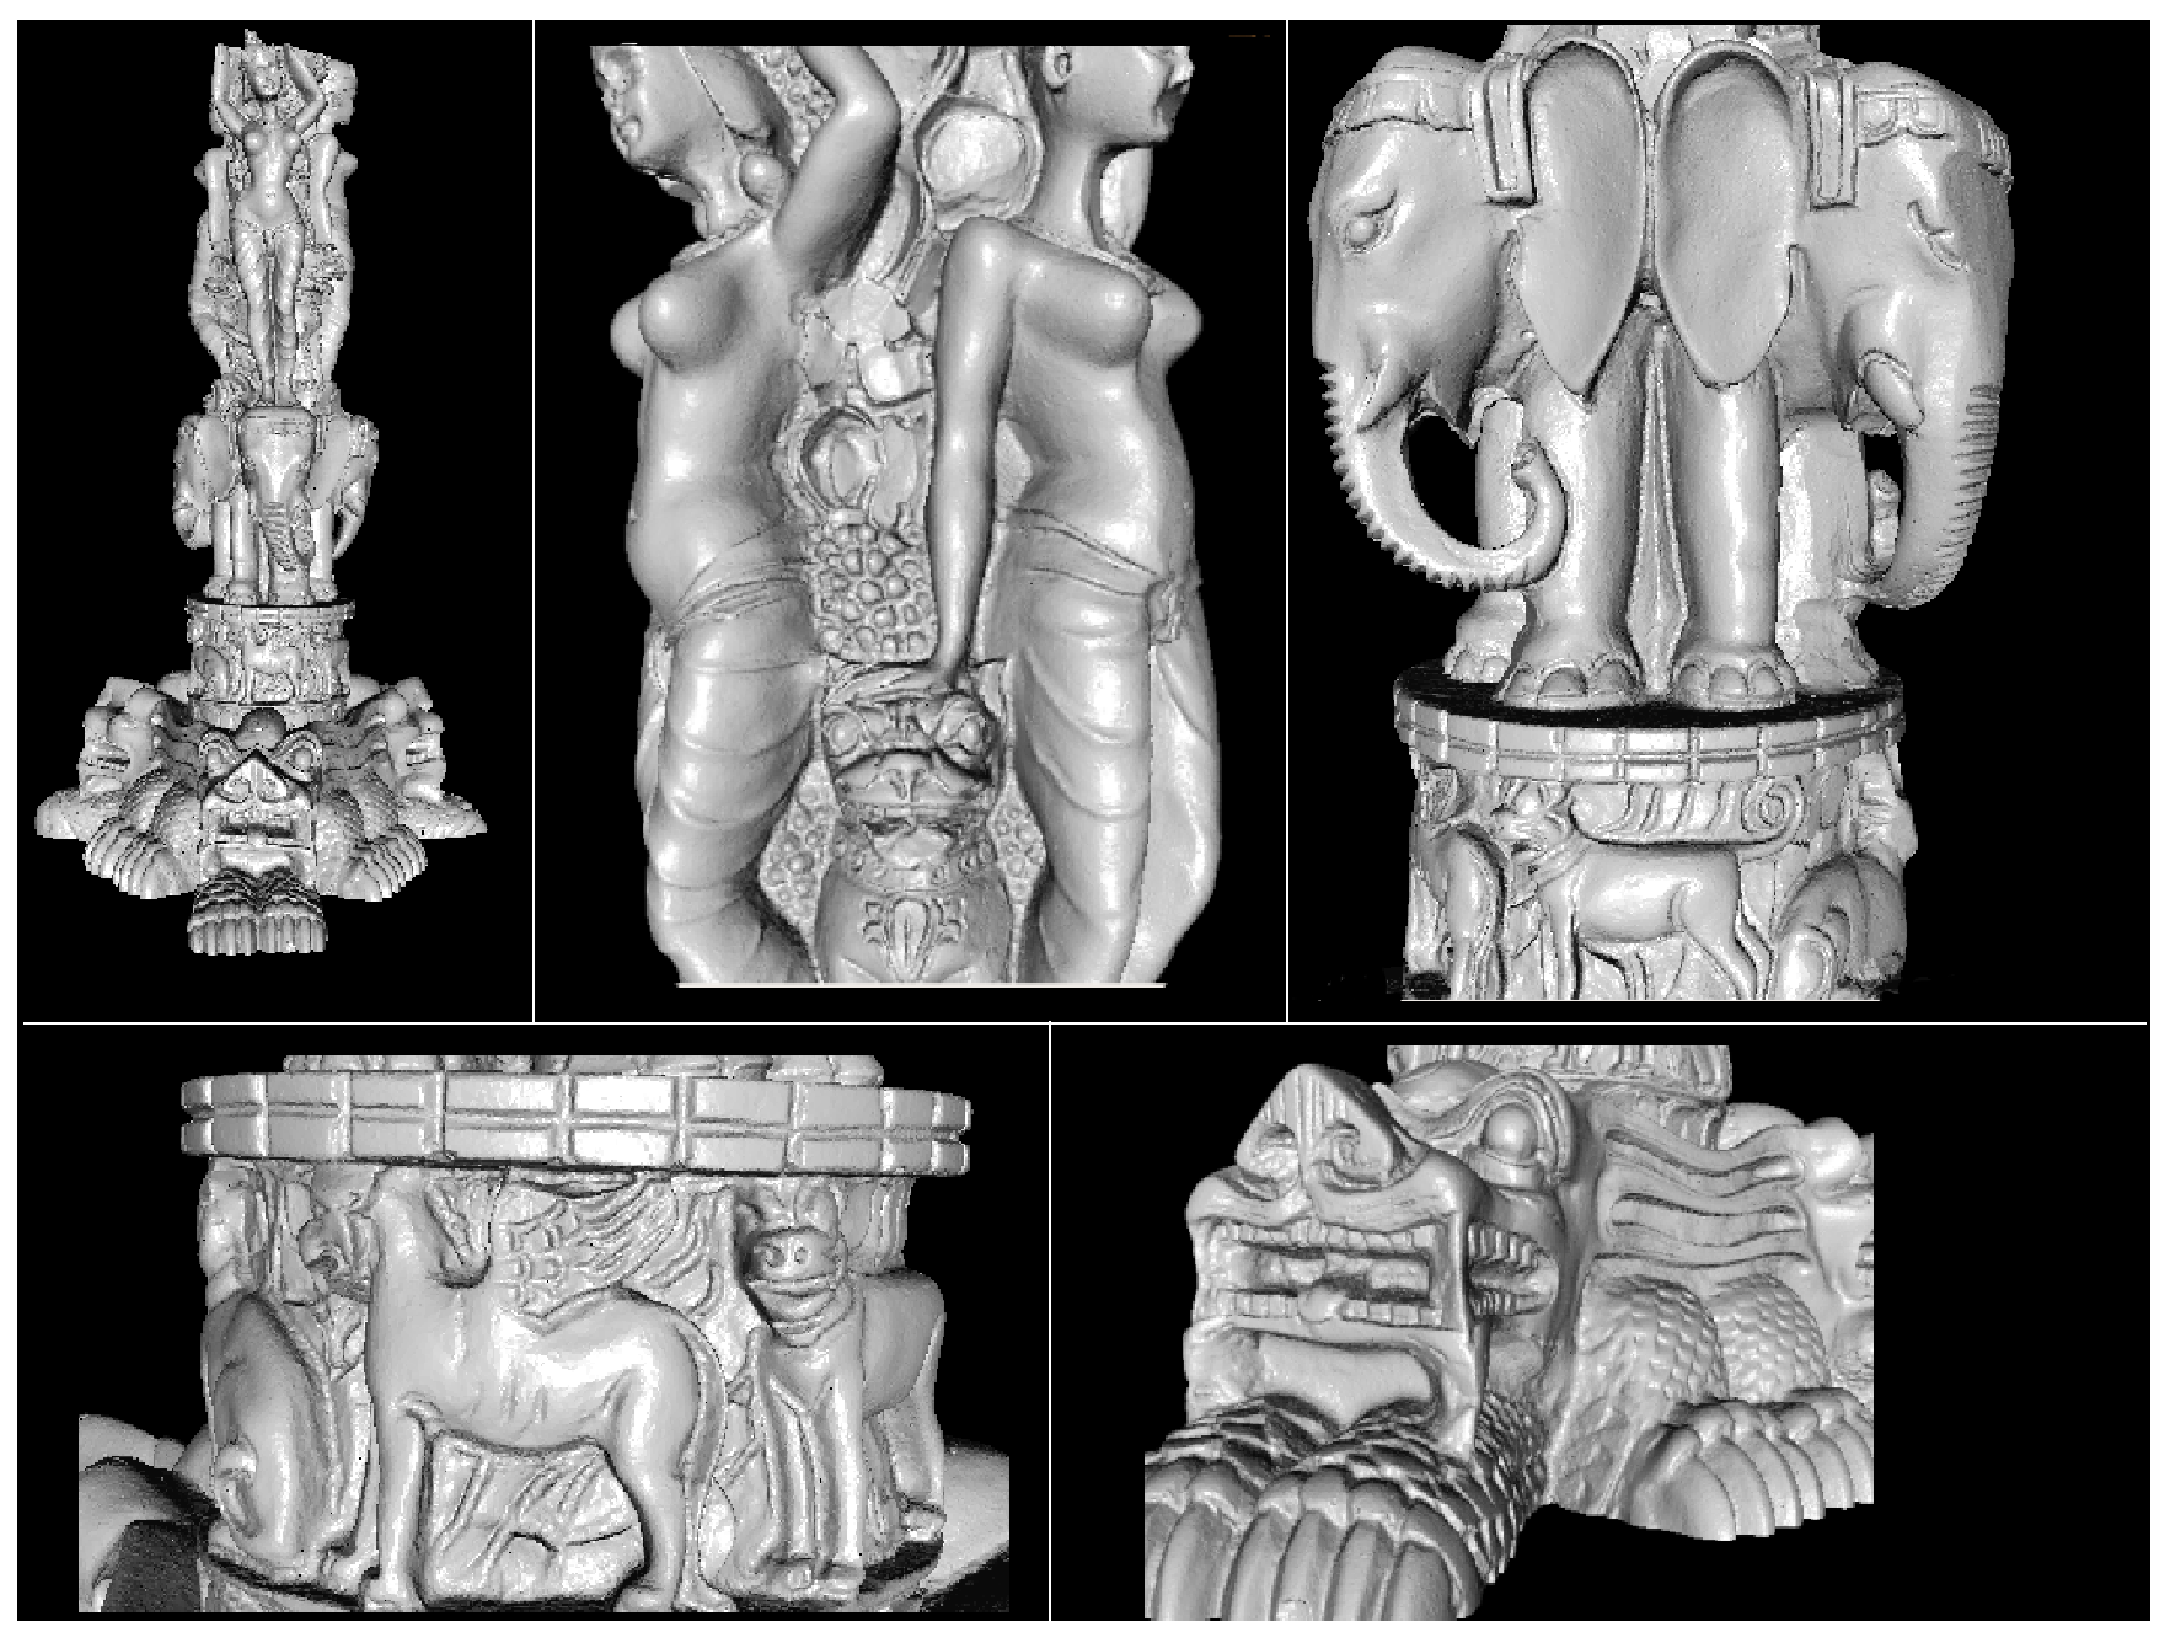
\epsfig{file=figs/thai, height = 0.6\textwidth} &
    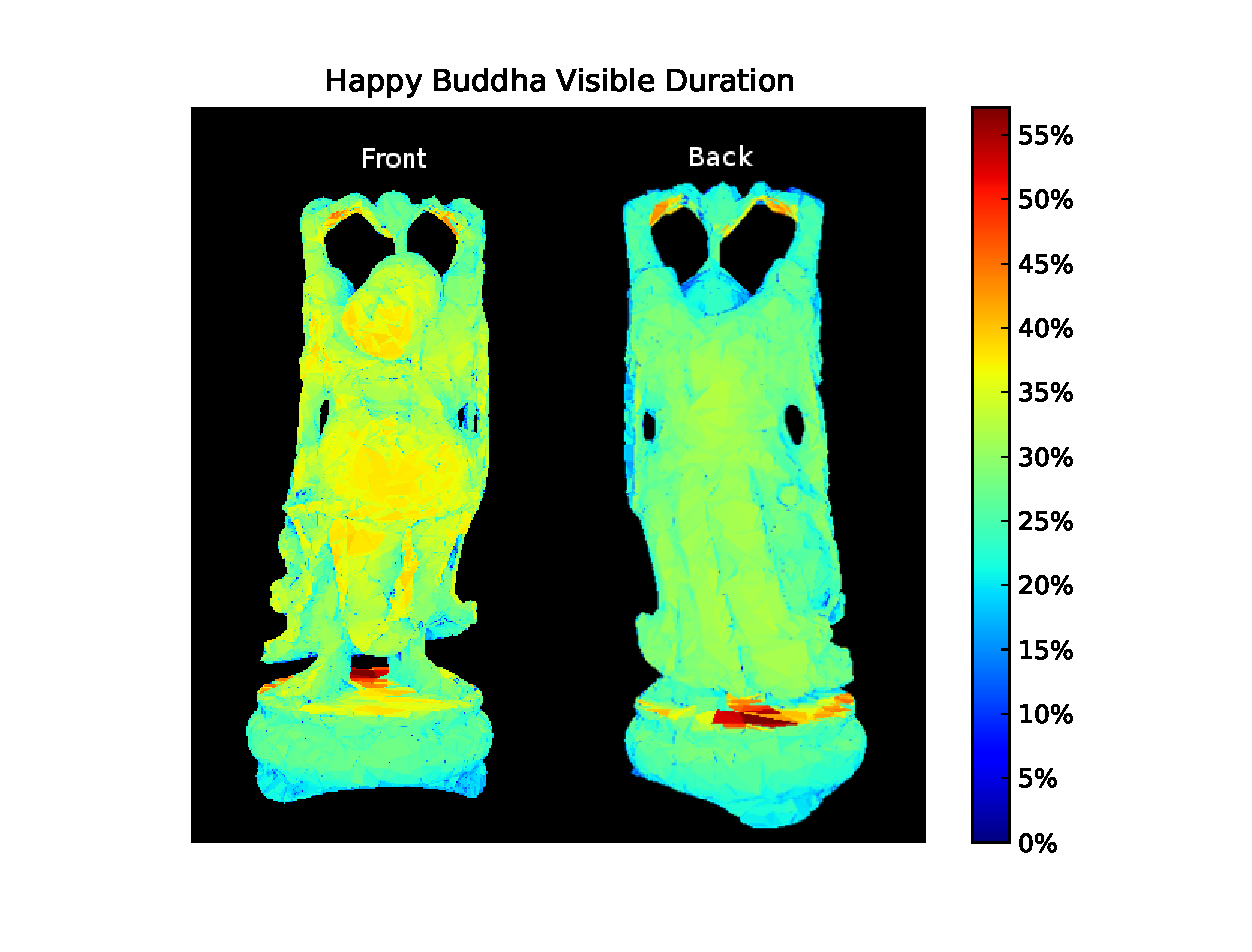
\epsfig{file=figs/happy, height= 0.6\textwidth} \\
    Thai Statue &
    Happy Buddha \\
\end{tabular}
\epsfig{file=figs/dragon, width = 0.7\textwidth} \\
Dragon
\caption{Meshes used in experiment.   
Thai Statue (5 million vertices), Dragon (3.6 million vertices), and Happy Buddha (0.5 million vertices).}
\label{fig:3dmodels}
\end{figure}

\section{User Study}
\label{s:user:study}
\textbf{Meshes}

Three 3D meshes are chosen from the freely available
Stanford 3D Scanning Repository\footnote{http://graphics.stanford.edu/data/3Dscanrep/}:
\textit{Happy Buddha}, \textit{Dragon}, and \textit{Thai Statue}.
These meshes vary in complexity (amount of vertices), orientation, and
symmetry in space from default viewing direction. \textit{Happy Buddha} is the
simplest, is vertically oriented, and has a default viewing direction
orthogonal from the face of the Buddha. From that direction, the mesh is
asymmetric between front and back. The geometric shape of \textit{Happy Buddha} is
somewhat representative of all human-like statues. \textit{Dragon} is more complex
and is horizontally oriented. The default viewing point is from one
side of the body. Unlike \textit{Happy Buddha}, it is front-back symmetric
relative to the default viewing direction. The geometric shape of \textit{Dragon} is
somewhat representative of most mammals. \textit{Thai Statue} is the most complex
and is actually a compound mesh composed of three identical sides, each 
with three different objects: a Goddess, an elephant, and a dragon,
stacking vertically from top to bottom.  These three sides connect to
form a triangular cylinder. There are three possible default
viewing directions, one each from three corners of the triangular mesh. The
\textit{Thai Statue} is included as an example of complex compound mesh.

We replicate each mesh above twice, generating nine meshes in total.  
We added one localized visual defect, by denting a small region, to each replicated mesh 
without changing its number of vertices or faces. The reason for adding the defects will be explained later. 
The location and nature of the
defects vary between the meshes. As \textit{Happy Buddha} is
relatively simpler and has a smooth surface, its defect is
 more obvious than \textit{Dragon}
and \textit{Thai Statue}.  Defects for the later two meshes, due to the
irregular surfaces, are hard to find unless the user zooms in
considerably.

The meshes are encoded progressively and streamed over a simulated network of 320Kbps and 400ms round trip time.  

\textbf{Participants.}

A total of 37 (25 male and 12 female) participants, aged 19 to 36
(mean 23), mostly from the university community participated in the
experiment. None had any visual handicaps.

\textbf{Design and Procedure}

Our experiment mimics the following general real world scenario. Customers
are shopping in an online antique store. Each product in the store has a
number of items, and each item is represented by a 3D mesh closely resembling
the corresponding real world item. These items vary in quality, and some
have visible defects. Before purchasing, customers will carefully examine the
available items for a product in order to pick the best item available for
that product category.

We designed our experiment using a simple case of the above scenario. 
Our online store has three different products,
corresponding to the three different meshes mentioned earlier. Each product
has three available items in varying quality. Two of them have visual
defects (note: defects are created without changing any mesh
characteristics). Due to the different complexity of each mesh, the defects
are easier to find in the simpler meshes (\textit{Happy Buddha}) compared to the more
complex ones (\textit{Thai Statue} and \textit{Dragon}).

\begin{figure}
    \centering
    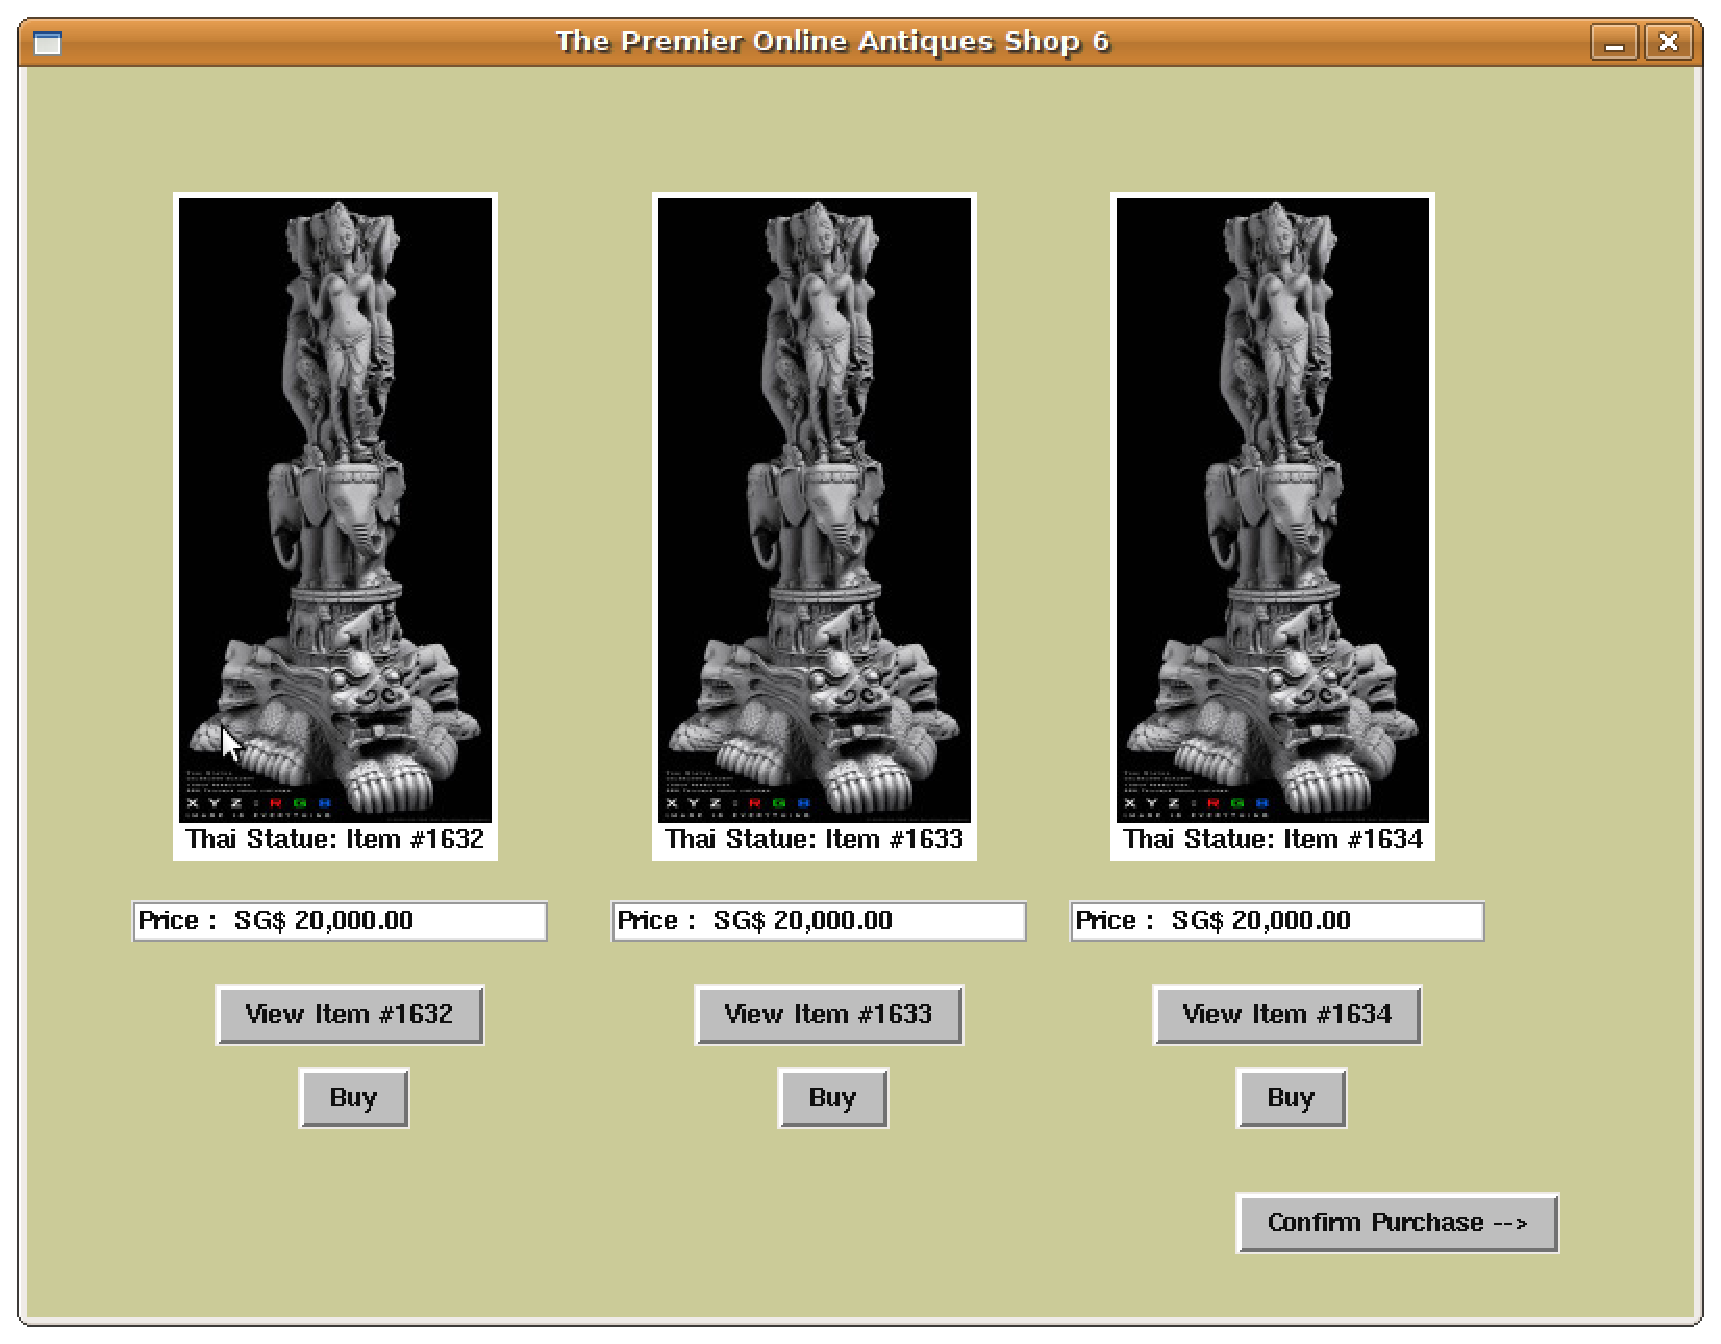
\epsfig{file=online_shop.eps, width = 0.85\textwidth}
    \caption{The user interface we used to mimick an online shop.}
    \label{f:user:shop}
\end{figure}
The participants were first instructed about the keyboard commands 
to view and interact with the 3D meshes, and given brief practice of
these commands on a simple mesh before starting the experiment. The
participants were presented with an user interface mimicking an online
catalog with three products (see Figure \ref{f:user:shop}).  For each product, images of three items 
(i.e., three versions, one original and two with defects) are shown on the screen.
The order of the products are randomized to avoid order effects.
The participants' job is to pick the best item among the three. Each item 
can be viewed in any order and if desired, multiple times.  When 
a participant selects an item, a new viewing window (width of 14cm and
height of 15cm, with a resolution of $500 \times 500$ pixels) opens, and the 3D mesh corresponding to that item is
progressively streamed and rendered in the window.  
The participants can interact freely
with the mesh until they close the window.
They would mark the item to be purchased after viewing all three items and
move on to the next product. Each participant must go through all three products to
complete the experiment.

\textbf{User Behavior Logs}

During the experiment, users' key press actions and viewpoints
were logged for off-line analysis. The representation of the viewpoints
and actions are introduced in detail as follows.

A viewpoint indicates from where and to which direction users view the mesh.
Users can change their viewpoints during the session. Changing the position of 
viewpoint is equivalent to changing the position of the mesh. 
%Therefore, from another aspect,
%users are changing the position and direction of the mesh during the session.
When the application starts, the user begins with the default viewpoint,
where the user looks at the center of the mesh (more precisely,  the center of the bounding box of the mesh)
from a distance far enough to see the whole mesh. 

We use a 6-tuple, ($x, y, z, \theta_x, \theta_y, \theta_z$) to indicate the relative position of the mesh,
%The ($x, y, z, \theta_x, \theta_y, \theta_z$) means
when the mesh is translated $x$ units right, $y$ units up, and $z$ units closer to the user (i.e. out of the screen),
and rotated $\theta_x$ degrees around $x$ axis, $\theta_y$ degrees around $y$ axis,
and $\theta_z$ degrees around $z$ axis. 
%During the rotation, the center of the mesh is not moved.
The positive directions of translation and rotation are shown in the Figure \ref{f:user:viewpoint}.
The default position is ($0, 0, 0, 0, 0, 0$).
\begin{figure}
    \centering
    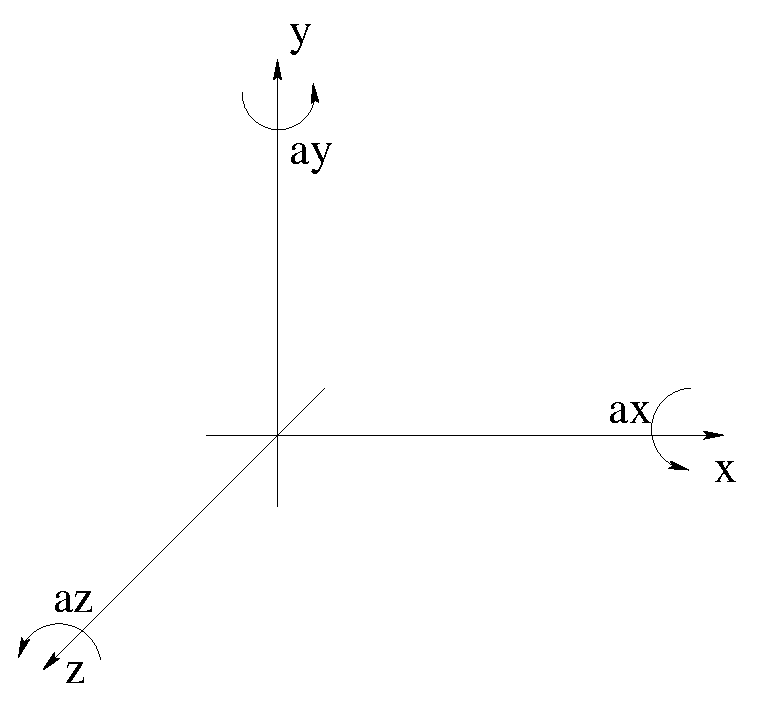
\epsfig{file=viewpoint.eps, width=0.3\textwidth}
    \caption{The positive direction of translation and rotation.}
    \label{f:user:viewpoint}
\end{figure}
The position of $x$, 
$y$, and $z$ changes in unit equivalent to one tenth of the bounding length, which is the edge length
of the bounding box of the mesh. The angles of $\theta_x$, $\theta_y$, and $\theta_z$ change in unit of 10$\degree$,
and their range is $[0, 1, \cdots, 35]$.

To facilitate the analysis, we ensure the six values are all integral. 
Therefore, an action will change one of the six values by one unit.
Table \ref{t:user:action} lists out the name, the abbreviation, the result,
and the corresponding key (or key combination) of each action.\footnote{
There is a small inconsistency in our design. 
We use $\uparrow$ to move the mesh closer and $\downarrow$ to move the mesh
further. It is more like moving viewpoint than moving the mesh. 
It is the flaw in our design, but fortunately the users were used to it quickly
during the experiments.}
%When moving and zooming, 
%we move the viewpoint of the user, 
%but when rotating, we rotate the mesh. 
%In other words, when we press ALT + $rightarrow$, 
%we move ourselves to the right side of the mesh. 
%When we press $rightarrow$, however, we revolve the statue to right. 
%Fortunately, users accept this setting well and without confusion.}.

\begin{table}
    \centering
    \begin{tabular}{|c|c|c|c|c|}
        \hline
        Name & Abbreviation & Result & key/key combination \\
        \hline
        move right & MR     & $x + 1$  & ALT + $\rightarrow$\\
        move left  & ML     & $x - 1$  & ALT + $\leftarrow$\\
        move up    & MU     & $y + 1$  & ALT + $\uparrow$\\
        move down  & MD     & $y - 1$  & ALT + $\downarrow$\\
        zoom in    & ZI     & $z + 1$  & $\uparrow$\\
        zoom out   & ZO     & $z - 1$  & $\downarrow$\\
        tilt backward & TB  & $\theta_x + 10\degree$ & CTRL + $\downarrow$\\
        tilt forward & TF   & $\theta_x - 10\degree$ & CTRL + $\uparrow$\\
        revolve anticlockwise & REAN & $\theta_y + 10\degree$ & $\rightarrow$\\
        revolve clockwise & RED & $\theta_y - 10\degree$ & $\leftarrow$\\
        rotate  anticlockwise & ROAN & $\theta_z + 10\degree$ & CTRL + $\leftarrow$\\\
        rotate  clockwise & ROC &  $\theta_z - 10\degree$ & CTRL + $\rightarrow$\\
        %reset      & RS     & $all = 0$  & R \\
        quit       & Q      & quit     & Q \\
        \hline
    \end{tabular}
    \caption{Introduction of the actions.}\label{t:user:action}
\end{table}


As a result, a user session can be seen as a random process 
with viewpoints as the states. Each action transits
the system from one state to next state, until the QUIT
action terminates the session (see Figure \ref{f:user:transition} as an example). 
During the session, we record
all the user actions and the time they happened.  We call these 
records \textit{user trace}.
Moreover, ($x, y, z, \theta_x, \theta_y, \theta_z$) can be seen as a point in a 6-dimension space, and
the six axises in this space are $X$, $Y$, $Z$, $AX$, $AY$, $AZ$. 
In this sense, a session is a random walk in the 6-dimension space.
\begin{figure}
    \centering
    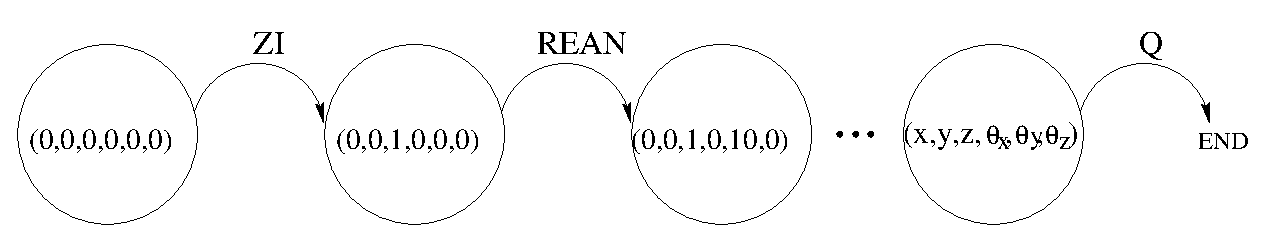
\epsfig{file=transition.eps, width=0.7\textwidth}
    \caption{An example of a user session}
    \label{f:user:transition}
\end{figure}


\section{Results and Implications}
In this section, we present our analysis on the user behavior. We present only on the analysis of the original (non-defect) statues, unless otherwise specified.
In addition, we also discuss what implications these results have on system design.

\subsection{Session Length}
\label{ss:user:session}
Session length refers to the time each user spends in viewing a mesh. 
Generally, the session length is short, with the average values of 107s, 76s, 47s for \textit{Thai Statue}, 
\textit{Dragon}, and \textit{Happy Buddha}, respectively (see Table \ref{t:TimeTable}). 
Figure \ref{fig:session-length}(a) shows the distribution. 
The session length decreases with complexity of the meshes, as expected. 
The session length fits the \textit{log-normal} distribution.

%The three models show different distributions. Such results are expected, for the session length is related to the users' interest in the models and the levels of details in different models.  Among these three models, Thai Statue is the biggest one, which provide the most coarse model to users when users start to view it, while ``Happy Buddha`` is the smallest one with less interesting details in it. 
%In generaly, the results of the session length distribution gives us two implications. First, the session length is short with maximum value of $376 sec$, which increase the difficulty in data sharing in P2P 3D mesh streaming systems. Second, the session length is dependent on the content of the models, and thus we need to consider the different features of the content of the model when generating synthetic traces for them.

\begin{figure}[htp]
\begin{center}
\begin{tabular}{cc}
\epsfig{file=figs/unconditionalThinkTimeResults/sessionLengthdistribution.eps, width=0.45\textwidth,angle=270}&
\epsfig{file=figs/unconditionalThinkTimeResults/Inter-operationTimeDistribution.eps, width=0.45\textwidth, angle = 270}\\
\end{tabular}
\caption{\label{fig:session-length} (a) Session Length and (b) Inter-stroke Time}
\end{center}
\end{figure}

%\begin{figure}[htp]
%\begin{center}
%\epsfig{file=figs/RegionType0/sessionLengthdistribution.eps, width=0.28\textwidth, angle = 270}
%\caption{The Session Length Distribution}
%\label{fig:session-length}
%\end{center}
%\end{figure}

\begin{table}[hbp!]
\begin{center}
\begin{tabular}{|c|c|c|c|c|c|}
\hline 
Mesh&\multicolumn{2}{c|}{Session Length}&\multicolumn{2}{c|}{Think Time}\\
\cline{2-5}
&Mean($s$)&Max($s$)&Mean($ms$)&Max($s$)\\
\hline
Thai Statue&107&376&593&25\\
\hline
Dragon&76&272&574&20\\
\hline
Happy Buddha&47&98&403&13\\
\hline
\end{tabular}
\caption{Session Length and Think Time\label{t:TimeTable}}
\end{center}
\end{table}%\begin{table}[hbp!]
%	\centering
%	  \caption{Session Length Stastistics}
%		\begin{tabular}{|c|c|c|c|}
%		\hline
%		Model&Sample Size&Mean(s)&Max(s)\\
%		\hline
%		Thai Statue&60&107&376\\
%		\hline
%		Dragon&63&76&272\\
%		\hline
%		Happy Buddha&39&47&98\\
%		\hline
%		\end{tabular}
%		\label{SessionTable}
%\end{table}

\subsection{Think Time}
\label{ss:user:thinktime}
We refer to the time between two key strokes as \textit{inter-stroke time}. 
Consecutive key strokes of the same type with inter-stroke time smaller than 20 $m$s
are grouped together as one \textit{action}. 
The time between two actions is \textit{think time}. 
We choose the threshold of 20 $m$s because there is an obvious gap between 5 $m$s and 35 $m$s
in the CDF of inter-stroke times for all meshes (see Figure \ref{fig:session-length}(b)).
%shows part of the inter-stroke time distributions. A gap exists between 5 $m$s and 35 $m$s approximately. 
%For larger values, the inter-stroke times follow similar distribution among different meshes. 
%Therefore, we select 20 $m$s as the threshold. 

%\begin{figure}[htp]
%\begin{center}
%\epsfig{file=figs/Inter-operationTimeDistribution.eps, width=0.28\textwidth, angle = 270}
%\caption{Inter-operation Time Distribution}
%\label{fig:interOpsTime}
%\end{center}
%\end{figure}
 
%The think time thus reflects the time interval between users' changing viewpoint. We study the think time distribution not only considering different models but also considering the different viewpoint regions of the model. 

%First, we give the results without considering the different viewpoint regions. 

We find that think time follows similar distributions for all of the three meshes (Figure \ref{fig:think-time}(a)). 
About 90\% of the think time is smaller than a second. There is a jump in the curve of think time distribution for all the three meshes -- 
about 5\% of the think time clusters around 0.5 seconds. 
We hypothesize that this is related to the 0.4-second round trip time in our experiments. 
After a user performs an action, it takes 0.4 seconds before the user can see progressive refinement of the mesh
(although the system responses to the change in viewpoint \textit{immediately}). 
Some users might wait for the refinement to come before the next action.

The mean and maximum think time are shown in Table \ref{t:TimeTable}. We note that the maximum is up to 50 times larger than the mean.

\begin{figure}[htp]
\begin{center}
\begin{tabular}{cc}
\epsfig{file=figs/unconditionalThinkTimeResults/ThinkTimeDistribution3.eps, width=0.45\textwidth, angle = 270}&
\epsfig{file=figs/conditionalThinkTimeResults1/ConditionalThinkTimeDistribution1hugenormal.eps, width=0.45\textwidth, angle = 270}\\
\end{tabular}
\caption{\label{fig:think-time} Think Time (x-axis in log scale).}
\end{center}
\end{figure}

To investigate the relation between think time and viewpoints, we
classify the viewpoints into 4 regions: front-far (FF), front-near
(FN), back-far (BF), and back-near (BN), based on \textit{front/back} and
\textit{far/near}. We find that the think time distribution is not
affected by the viewpoint (see Figure \ref{fig:think-time}(b)). 

Next, it is reasonable to assume think time is small when user just repeat 
the previous action and the think time tends to be big when user change to another action.
Figure \ref{f:user:thinktime} shows this assumption is correct.
\begin{figure}
    \centering
    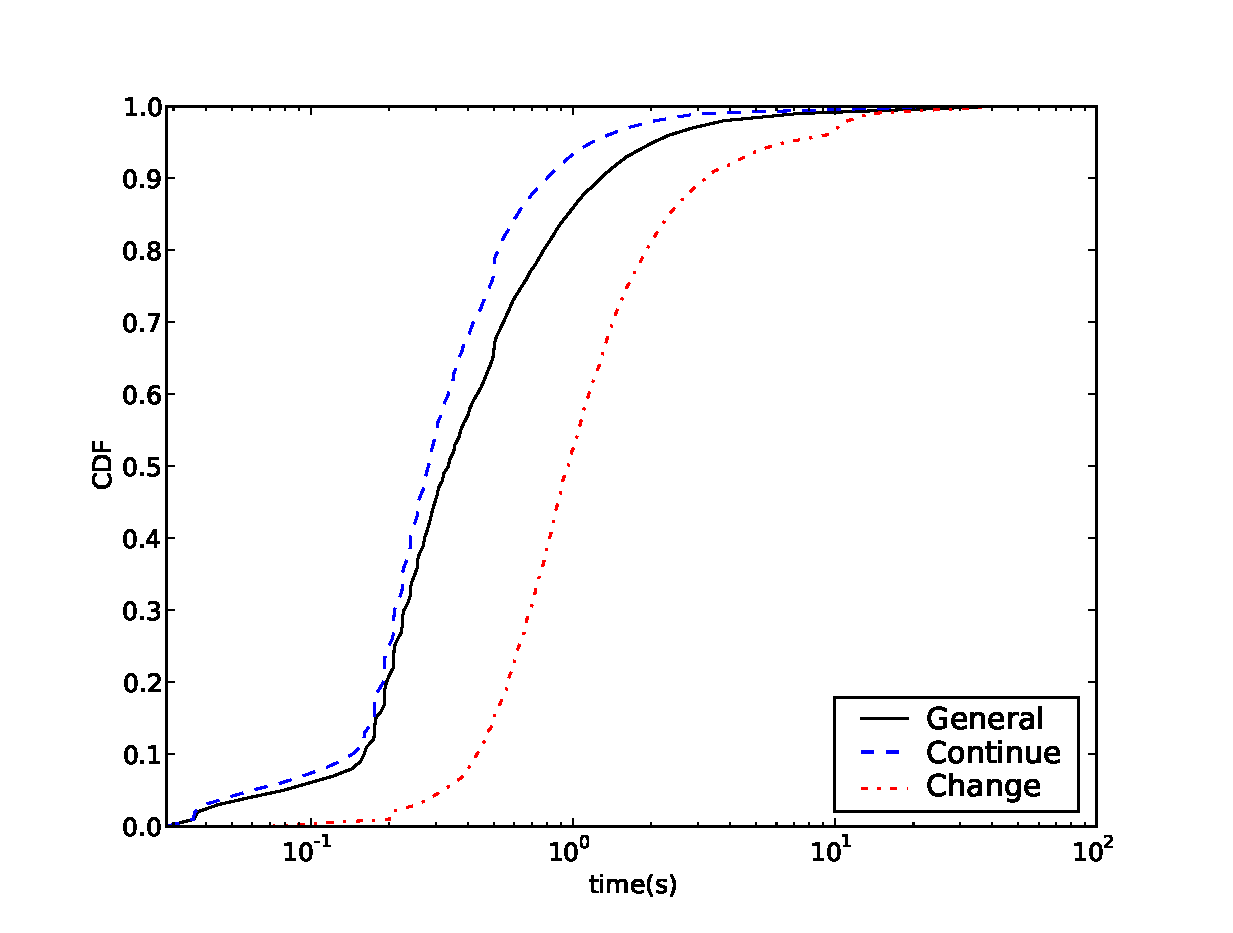
\epsfig{file=thinktime.eps, width=0.5\textwidth}
    \caption{Think time is smaller when user repeat the previous action.}
    \label{f:user:thinktime}
\end{figure}

\subsection{Access Pattern}
Proxy caching of meshes is useful in reducing the service load.  
In this section, we show that the user traces exhibit access
patterns that can lead to efficient caching.

\textbf{Caching for Mesh Streaming}.
In progressive mesh streaming, vertex splits are often grouped into chunks
for transmission. These chunks can be cached at a proxy to reduce server overhead.
To study the usefulness of proxy caching, we look at the access pattern to chunks. 

We first replay the log of actions from the users, and generate
a list of chunks accessed  by users during the experiment.  
From these chunk traces, we count
the number of times each chunk 
is accessed.  We then sort the chunks 
in decreasing order of the access count, and plot the cumulative
access count versus rank in Figure \ref{fig:CDF}(a).  We
normalize both axes to between 0 and 1 so that we can plot
all three meshes on the same graph.  
Figure \ref{fig:CDF}(a) shows how many requests we can satisfy (i.e., hit rate) 
by storing the most frequently requested chunks in a proxy. 
The x-axis denotes the number of chunks stored in the proxy, 
as a fraction of total number of chunks requested
(note: not the total number of all chunks).
It can be observed that by building a static
cache that stores 20\% of the most frequently accessed
chunks, the proxy can achieve more than 70\% hit rate for
\textit{Thai Statue} and \textit{Dragon}, and 55\% for 
\textit{Happy Buddha}.

    \begin{figure}[htp]
        \begin{center}
        \begin{tabular}{cc}
            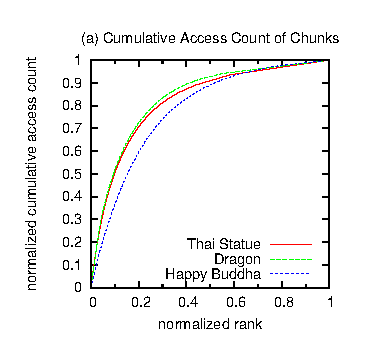
\epsfig{file=RequestCountCDF2.eps, width = 0.45\textwidth}&
            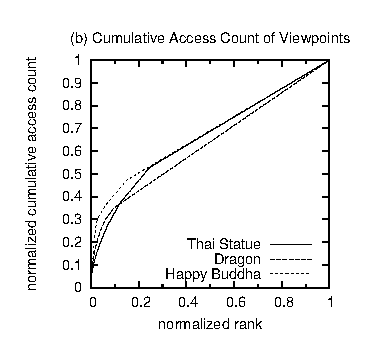
\epsfig{file=vpCDFpercentage.eps, width = 0.45\textwidth}\\
        \end{tabular}
    \end{center}
        %\caption{Normalized cumulative access count of mesh (left: chunks, right: pre-rendered images) versus rank.\label{fig:CDF}}
        \caption{Cumulative Access Count versus Rank\label{fig:CDF}}
    \end{figure}

\textbf{Caching of Remote Rendering.}
For rendering on mobile devices \cite{bao06remote} or for 
protection of mesh data \cite{koller04scanview}, 
the server could send a rendered image directly according to the users' viewpoint.
In this
scenario, the caching proxy can cache the rendered images.  We can
similarly find the viewpoints ``visited'' by the most users.  A
viewpoint visited multiple times by the same user is only counted
once, since the user can keep the received image locally and need not
request it the second time.  Figure \ref{fig:CDF}(b) shows a plot
similar to Figure \ref{fig:CDF}(a), but for access frequency of 
viewpoints.  The figure shows the hit rate at the caching proxy 
if we choose to store pre-rendered images corresponding to the
most frequently accessed viewpoints.
The distribution is not as skewed as access count for chunks, 
but still, caching the rendered images for 20\% of the most 
frequently accessed viewpoints can yield 40 - 50\% hit rate.

\textbf{Caching of Vertices and Pixels.}
Caching mesh data in graphic card memory 
(e.g. using VBO (Vertex Buffer Object) and PBO (Pixel Buffer Object) supported in OpenGL), 
could significantly increase the rendering speed when the memory bandwidth is the bottleneck.
For graphic cards without enough memory to store the whole mesh, we could just store the most frequently viewed part of the mesh
in the graphic card memory. 
%Since changing the stored data in graphic card memory is usually expensive, so 
%the stored data cannot be adaptively changed.

We replay all the user traces, and whenever the viewpoint changes 
%count the number of times each face is viewed.
we add the access number of the visible faces by one. 
Therefore, the access number of a face is the count of viewpoints at 
which it is visible (revisiting to a previously visited viewpoint is also counted
since the mesh will still be rendered). 
We normalized the number of views of each face and visualize them with
 a heat map (Figure \ref{fig:heat_map}). 
%duration of different parts of the ``Happy Buddha'' mesh obtained by
%replaying all the traces we collected.  
We can see that the most frequently viewed region of \textit{Happy Buddha} (viewed 4205 times) is 
the base between the two legs because it is visible from both the front and the back.
%Next, we sort the faces in decreasing order of the access count, and draw 
Figure \ref{fig:face_hit_rate} plots the normalized cumulative view count of faces versus rank, 
similar to Figure \ref{fig:CDF}. We can see that the locality is slightly less than
that in the previous two scenarios, but for \textit{Happy Buddha} and \textit{Thai Statue}, hit rate of 40\%  can be achieved
%accesses can be satisfied 
by storing 20\% of the most frequently viewed faces in the graphic card memory.
The mesh \textit{Dragon} has the least locality. We hypothesize that this is because %related to two reasons:
people tend to view \textit{Dragon} at many different viewpoints due to its complex shape,
%Hence, it is relatively less common for users to come back to viewpoints previously visited. 
leading to more evenly distributed viewpoints around the mesh.
%and faces have even chances to be viewed.
%    \begin{figure}[htbp]
%        \centering
%        \begin{tabular}{cc}
%        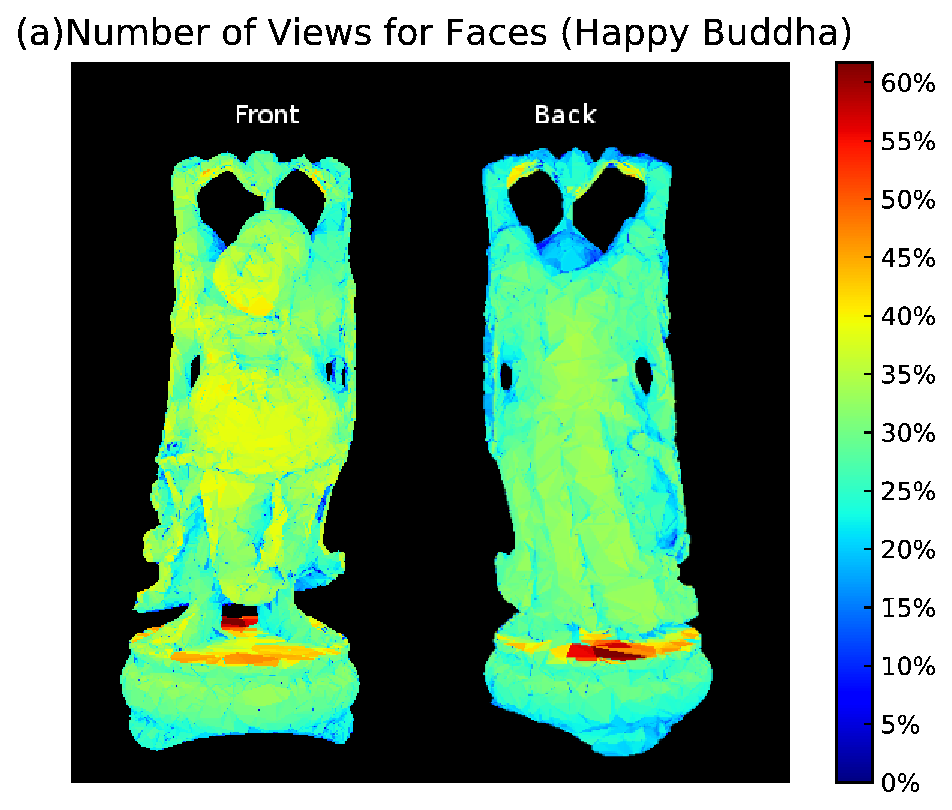
\epsfig{file=heatmap2.eps, width =0.5\textwidth}&
%        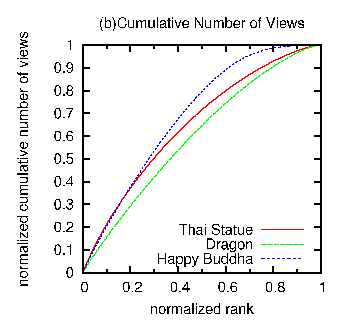
\epsfig{file=faceCache.eps, width = 0.5\textwidth}\\
%    \end{tabular}
%        \caption{(a)The normalized number of views for each face. (b) The hit rate when we save part of the faces in the graphic card.\label{fig:heat_map}}
%    \end{figure}
    
\begin{figure}[htp!]
    \centering
\begin{tabular}{c}
 \epsfig{file=heatmap_buddha_bw.eps, height=0.45\textwidth} \\
 \epsfig{file=heatmap_dragon_bw.eps, height=0.45\textwidth} \\
 \epsfig{file=heatmap_thai_bw.eps,   height=0.45\textwidth} 
\end{tabular}
\caption{The normalized number of views for each face. \label{fig:heat_map}}
\end{figure}

\begin{figure}[htdp!]
    \centering
 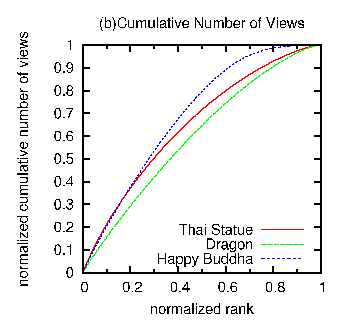
\epsfig{file=faceCache.eps, height=0.45\textwidth}
\caption{The hit rate when we save part of the faces in the graphic card.\label{fig:face_hit_rate}}
\end{figure}

\subsection{Predictability}
\label{ss:user:predictability}
Besides the session length, think time, and the access pattern,
it is also interesting to see if user actions are predictable. 
If so, pre-fetching can be used to reduce response time when
users change their viewpoints. For example, when the connection between the 
receiver and the sender has limited bandwidth
or long delay, the requests for vertex splits of the new viewpoint 
can be sent based on the prediction before the user changes the viewpoint.
Another example is that when the client has limited
rendering power, the next viewpoint can be rendered
in advance based on the prediction to reduce the response time. 
%In both cases, the accuracy of the prediction is important.

The next action of a user, $A_n$, is a random variable with 14 possible values
(see Table \ref{t:user:action}). 
A naive way to predict the value of $A_n$ is based on the unconditional distribution 
of $A_n$, which can be estimated as the frequency of each value in the traces
we collected.  
Then the $A_n$ can be predicted as the action with highest probability.
Figure \ref{f:user:frequency}
shows the frequency of occurrences of 12 different actions.
%\footnote{We ignore RESET and QUIT 
%in this figure because they have the lowest probability.}
on the traces from each of 9 meshes,
displayed as a bubble chart. 
The bubble size indicates the frequency of an action occurring for a mesh.
We can see that the most frequently used actions are two revolving (rotating around y-axis). 
As a result, without any extra information, we can always predict that the next action is 
one of the two revolving.
The accuracy of this prediction, however, is low. 
Take the Thai mesh as an example,
the accuracy is $33.07\%$. % if we guess one action and $64.34\%$ if we guess two actions
%(if the real action is one of the predictions, we consider our prediction is accurate).
The prediction could be more accurate with more information,
such as the previous action of the user and the current viewpoint of the user.
\begin{figure}[htdp!]
    \centering
    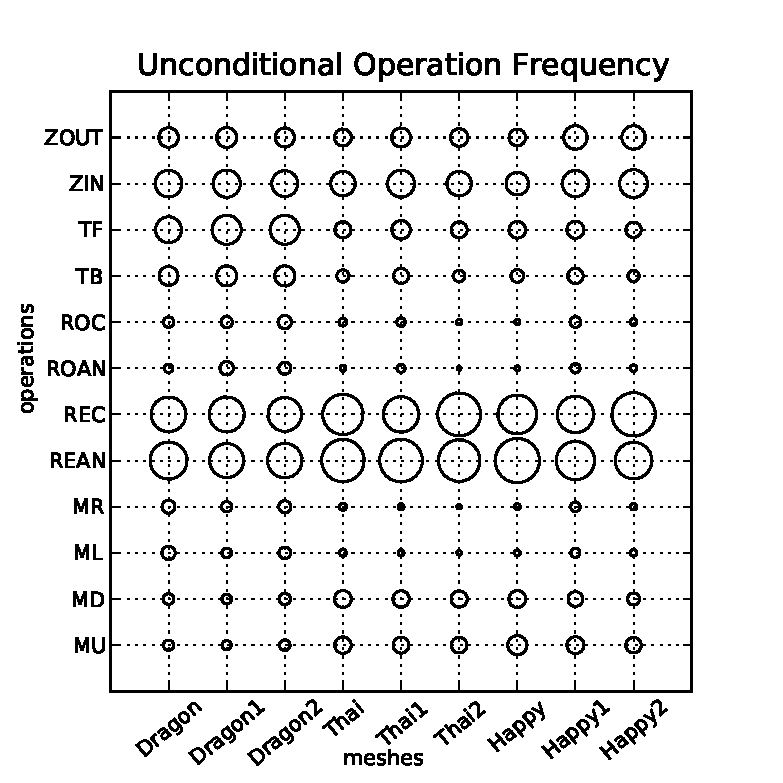
\epsfig{file=UnActionEventFrequency.eps, width=0.45\textwidth}
    \caption{The frequency of 12 actions in the traces we collected.}
    \label{f:user:frequency}
\end{figure}

\textbf{Considering Previous Action}

From the traces we found that the value of $A_n$ highly correlates
with the value of $A_p$, the previous action taken by the user.
Figure \ref{f:user:prev_next_relation} shows the conditional 
probability of taking the next action given the previous action
%for \textit{Thai Statue}.
for the three meshes.
The shaded diagonal shows that the same action has the 
significantly larger probability (e.g., more than 0.93 for revolving) 
of being taken next. %The other meshes exhibit the similar pattern. 
\begin{figure}[htp!]
    \centering
    \begin{tabular}{c}
        \epsfig{file=figs/traceHistogram0/Inter-operationprobability-hugenormal.eps, width=0.45\textwidth}\\
        \epsfig{file=figs/traceHistogram0/Inter-operationprobability-dragonnormal.eps, width=0.45\textwidth}\\
        \epsfig{file=figs/traceHistogram0/Inter-operationprobability-happynormal.eps, width=0.45\textwidth}
    \end{tabular}
\caption{The conditional probability of next action if the previous action is given.}
\label{f:user:prev_next_relation}
\end{figure}

According to this observation, 
we categorized the actions into two types: \textit{repeat}, \textit{non-repeat}. 
Then we can predict the next action by choosing ``repeat'' unconditionally.
The probability of ``repeat'' for three meshes can be seen in Figure \ref{f:user:cont_prob}.
Therefore, always choosing ``repeat'' as the prediction has high accuracy 
(larger than $80\%$ for all meshes). 
\begin{figure}[htdp!]
    \centering
    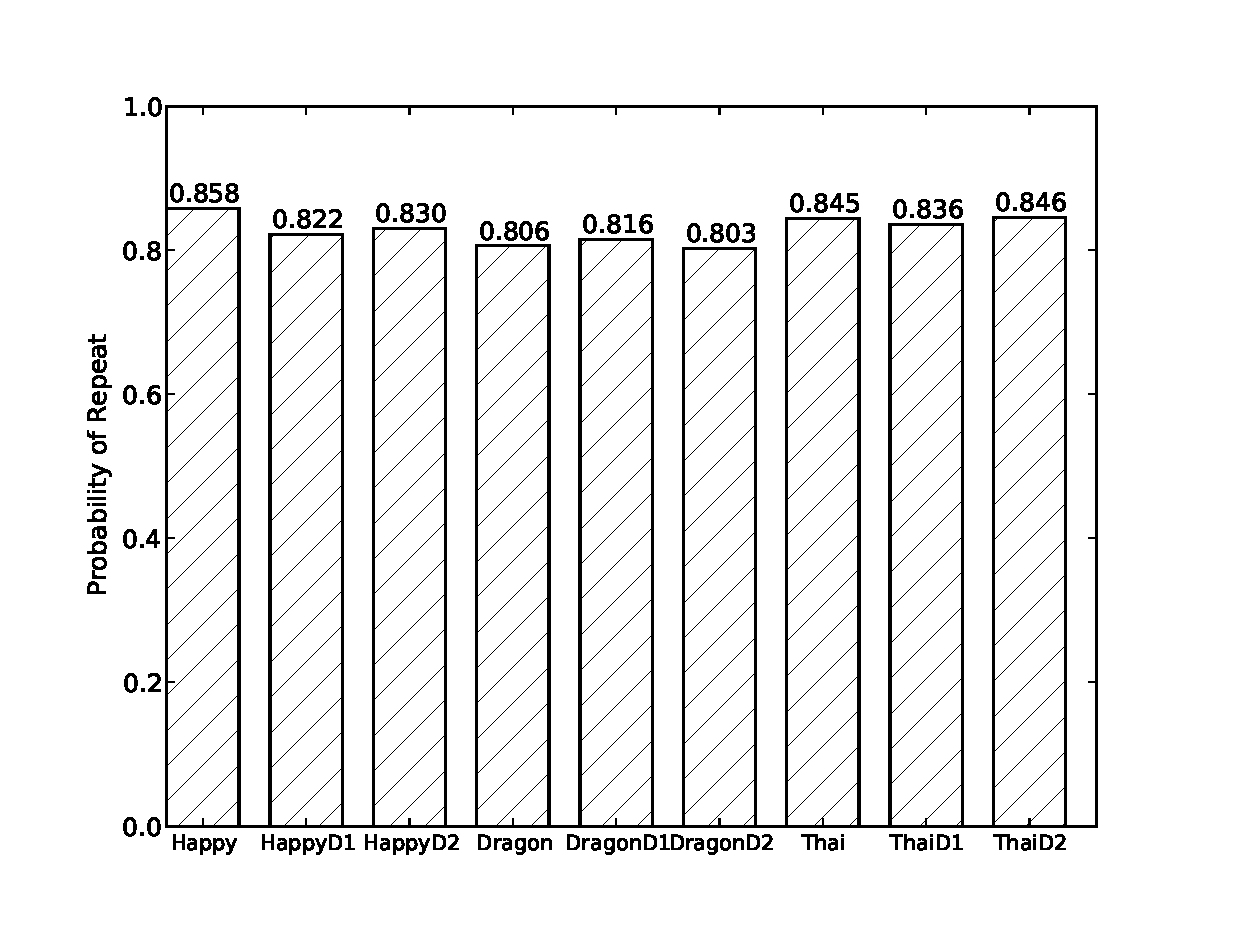
\epsfig{file=cont_prob_9.eps, width=0.6\textwidth}
    \caption{The probability of repeating the previous action for 9 meshes.}
    \label{f:user:cont_prob}
\end{figure}

\begin{figure}
    \centering
    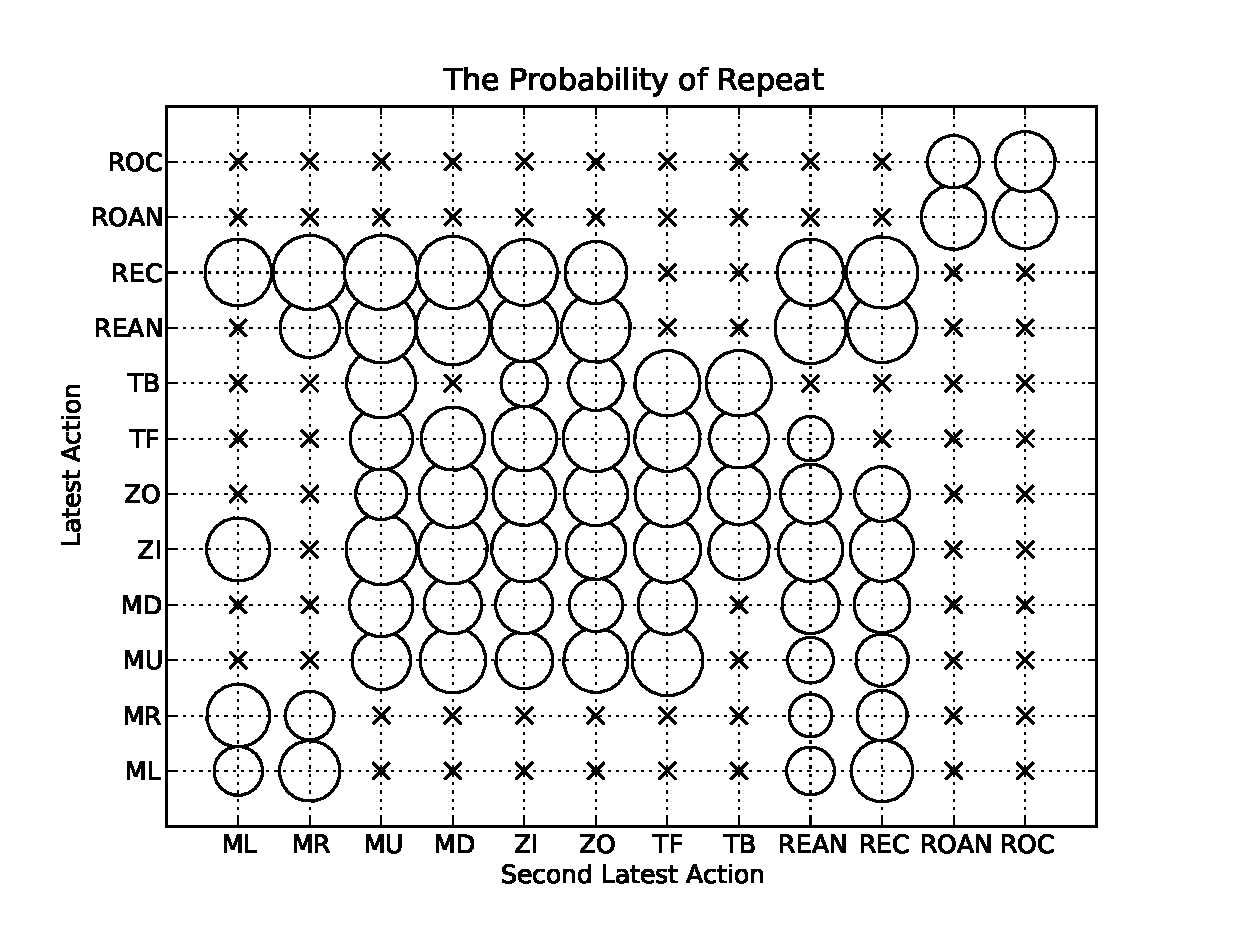
\epsfig{file=happy_2.eps, width=0.55\textwidth}\\
    Buddha\\
    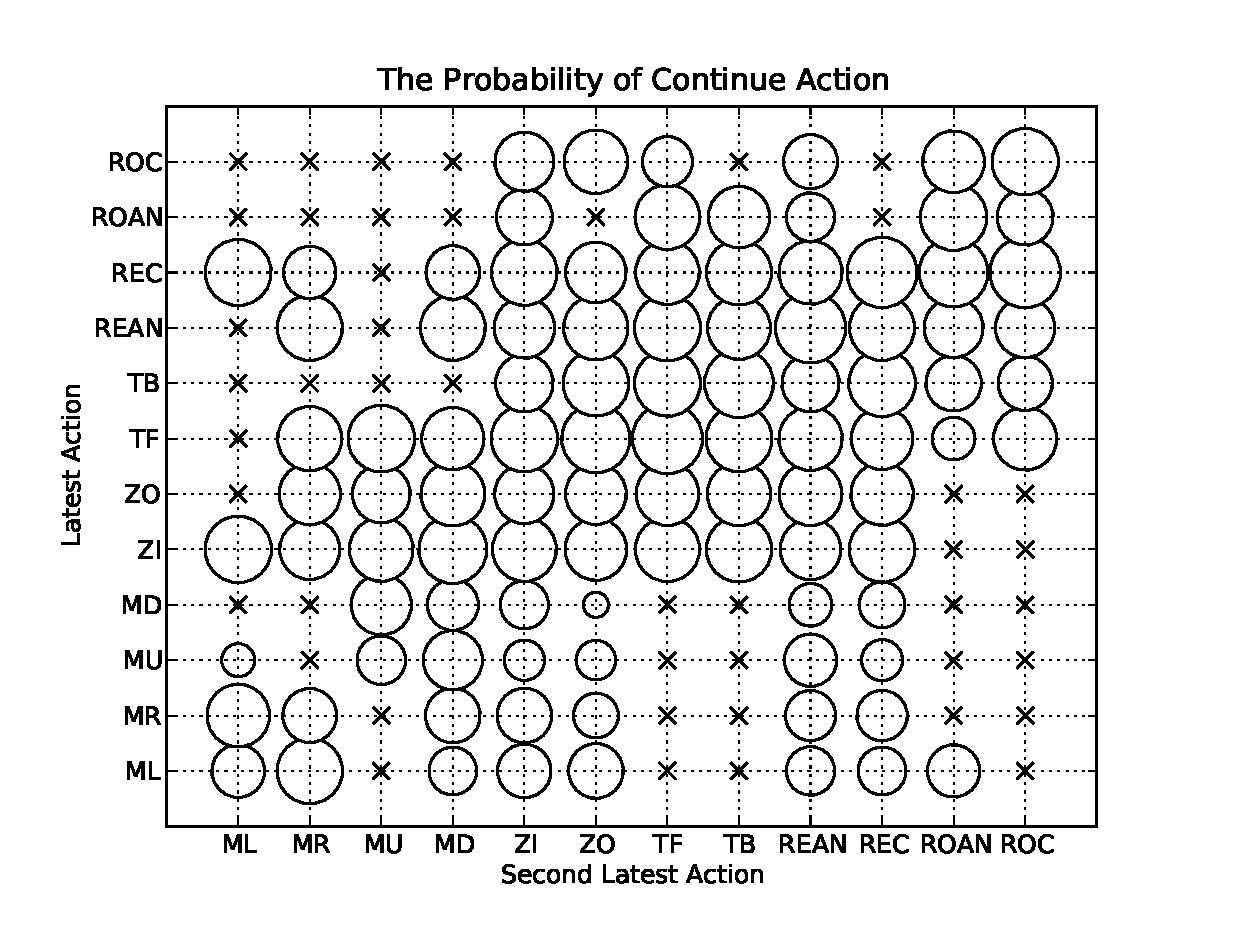
\epsfig{file=dragon_2.eps, width=0.55\textwidth}\\
    Dragon\\
    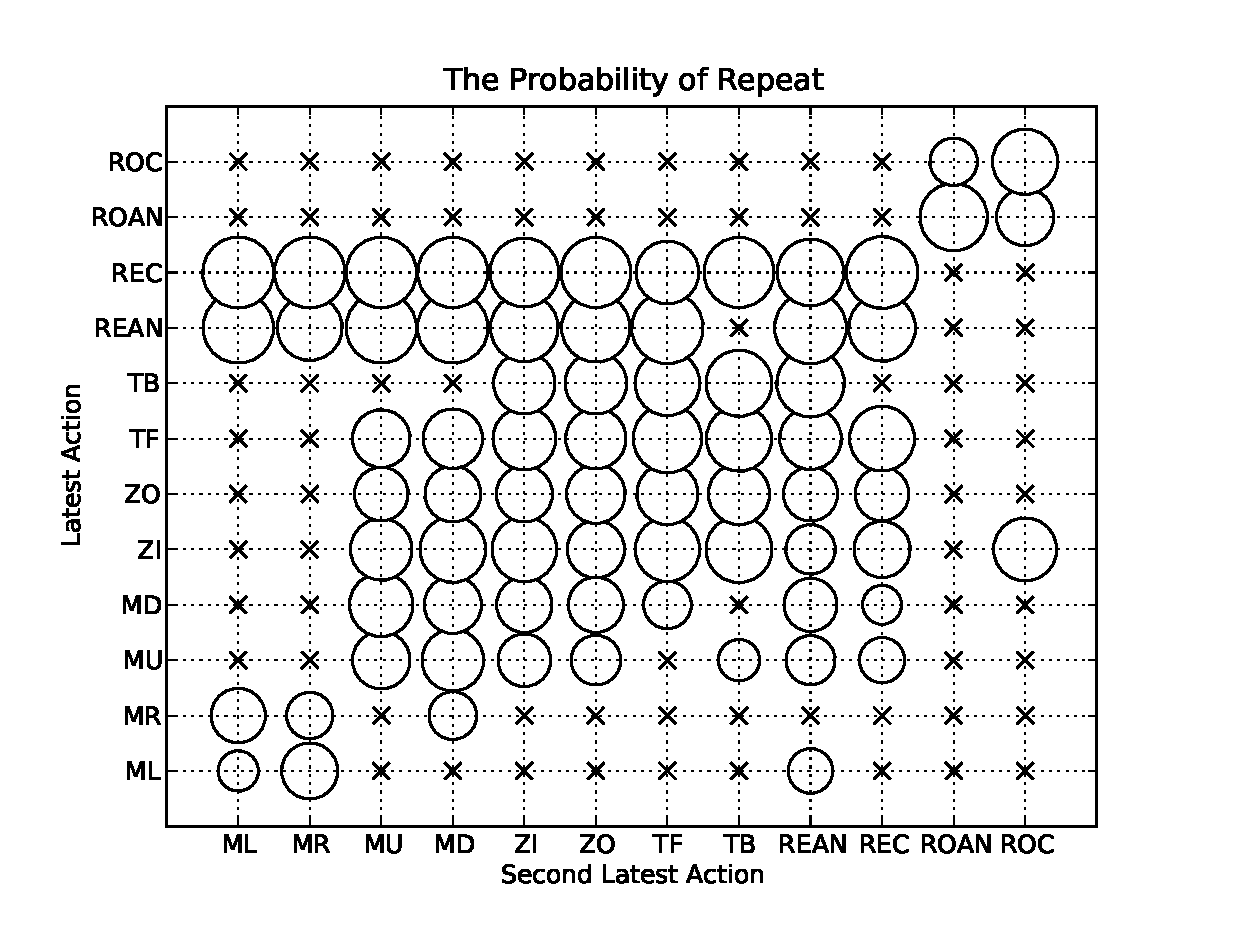
\epsfig{file=thai_2.eps, width=0.55\textwidth}\\
    Thai Statue
    \caption{The probability of repeating the previous action for each combination of previous two actions (Thai Mesh).
    'x' means that the sample size of this combination is too small (less than 10 samples) to obtain reliable probability.}
    \label{f:user:prev2}
\end{figure}
Next, we check whether it helps to consider one more action, the second latest action. 
The probability of repeating the previous action under different combination of
previous two actions for Thai Mesh is shown in Figure \ref{f:user:prev2}.
In this figure, we can see that the second latest action does affect the 
repeat probability, but the effect is much less significant than the previous action. 
Moreover, we found that in around 99.9\% of the combinations, 
repeating the previous action still has the largest probability,
so the prediction based on previous action and the one based on previous two actions are the same in
most of the cases. 
Therefore, we conclude that considering only the previous action is enough for the prediction.

\textbf{Considering Viewpoint}

The other method to improve the prediction accuracy is to consider the current viewpoint of the user.
We compute the conditional distribution of next action $A_n$ on each viewpoint, 
and always choose the action with the highest conditional probability as the prediction.

Since we estimate the probability of an action as the frequency 
of its occurrence in the real traces, 
enough number of samples are required to give reliable results. 
By analyzing the traces we collected, we found that majority of the samples are 
on a small proportion of viewpoints, and for the rest viewpoints, we have few
samples (See Figure \ref{f:user:sample_size_1}).
\begin{figure}
    \centering
    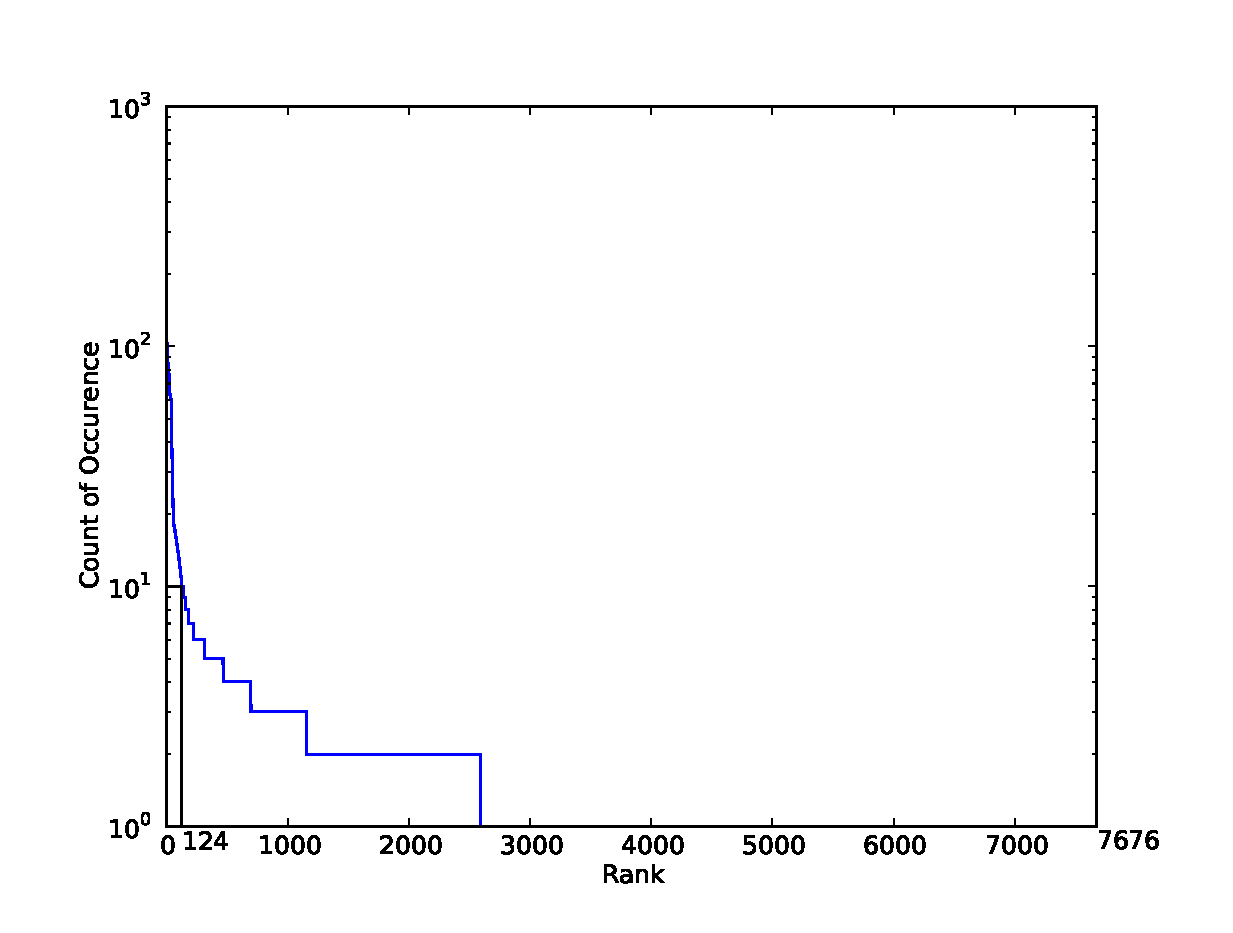
\epsfig{file=happy_sample_size_1.eps, width=0.55\textwidth}\\
    Buddha\\
    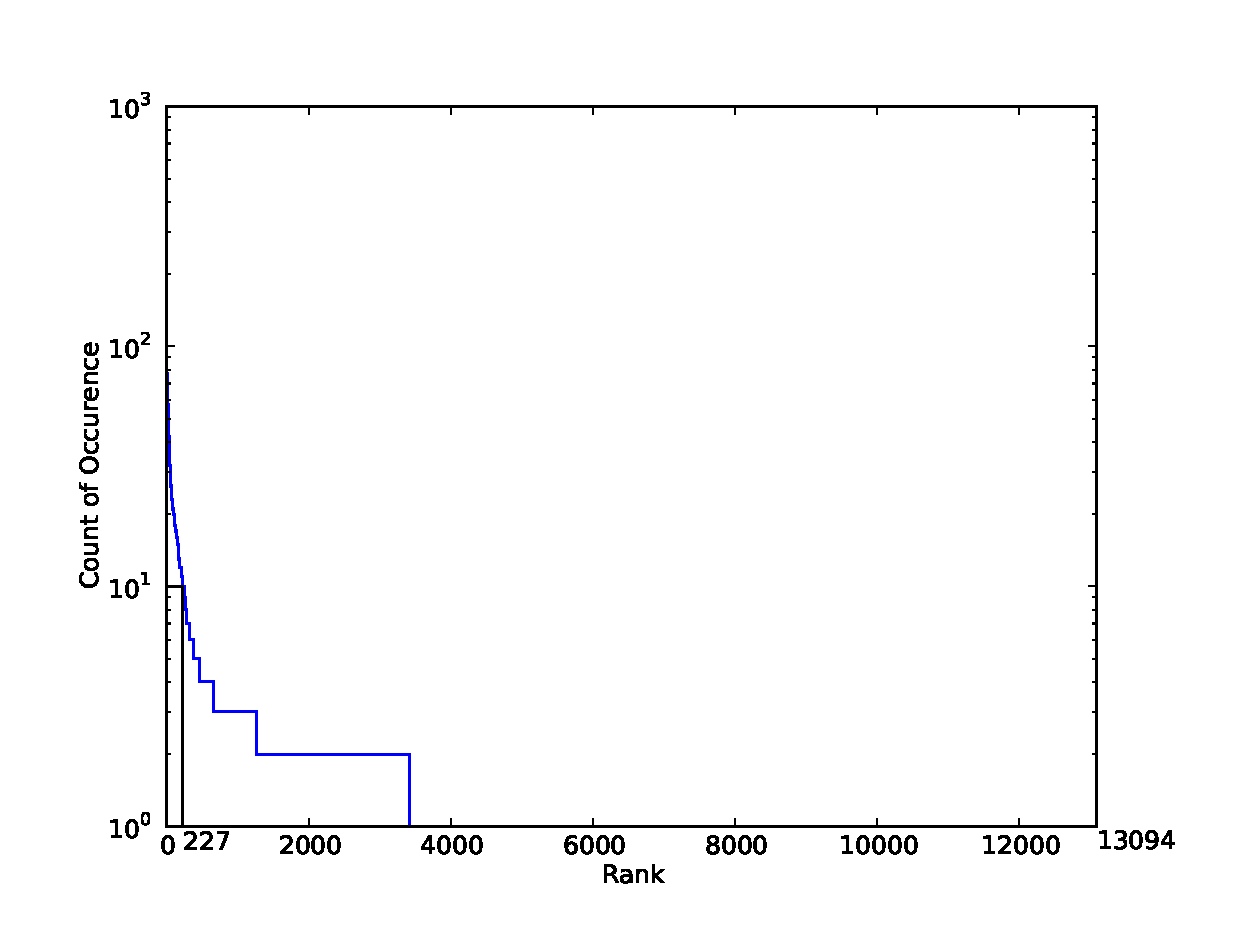
\epsfig{file=dragon_sample_size_1.eps, width=0.55\textwidth}\\
    Dragon\\
    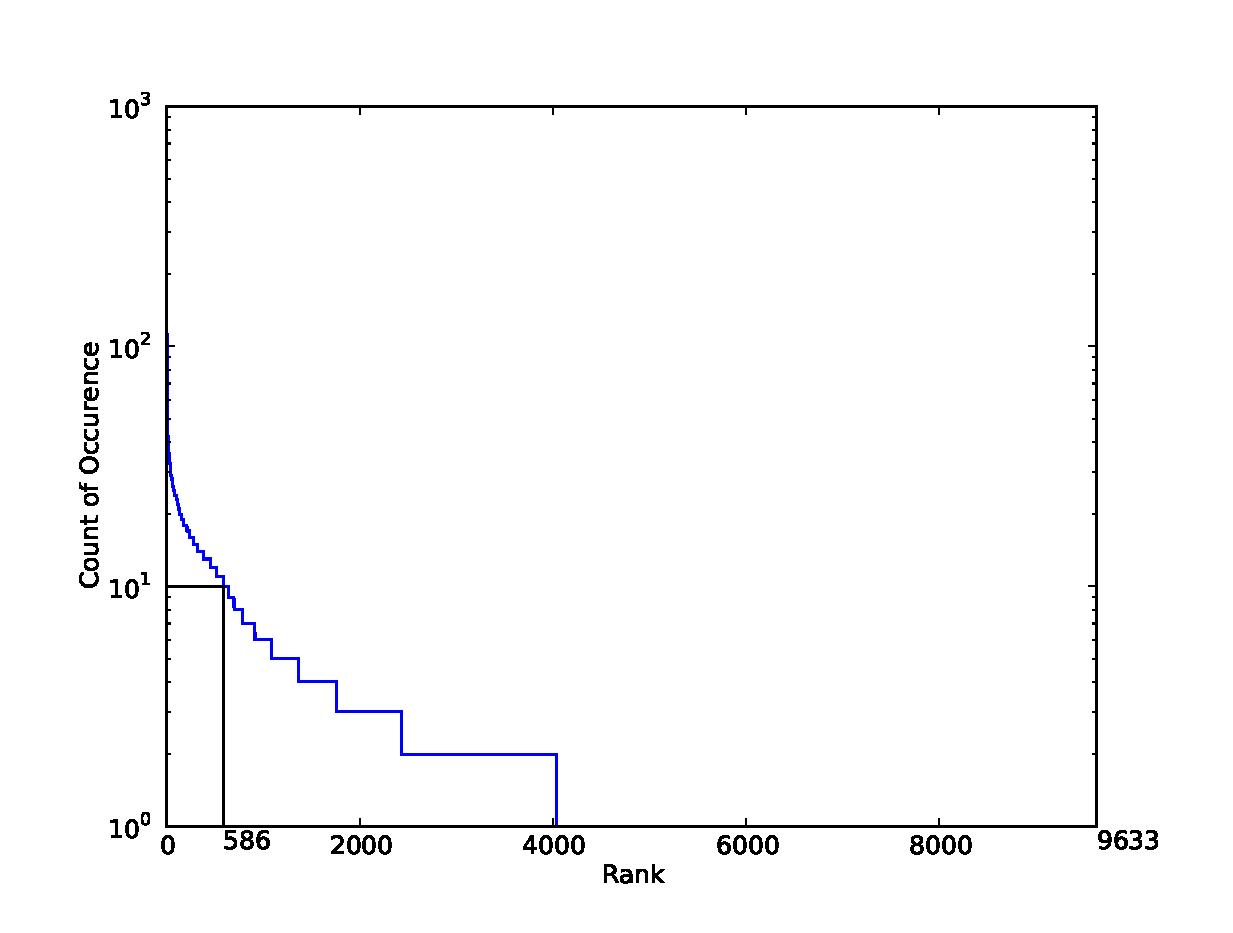
\epsfig{file=thai_sample_size_1.eps, width=0.55\textwidth}\\
    Thai Statue
    \caption{The number of samples on all viewpoints, and the viewpoints are sorted from the most popular to the least popular.}
    \label{f:user:sample_size_1}
\end{figure}
Including the viewpoints having few samples may exaggerate the accuracy.
For example, the predictions on all the viewpoints having one sample are 
always 100\%, which is not realistic.
Therefore, we ignore all those viewpoints with less than 10 samples.
The accuracy of this method can be seen in Figure \ref{f:user:accuracy_comp} (labelled ``Vp'').
We can see that this method has lower accuracy than the one based on previous action.

\textbf{Considering Viewpoint and Previous Action}
To improve the accuracy, we could consider both viewpoint and previous action.
%Now we consider both current viewpoint and  previous action.
Similarly, we compute the conditional distribution of next action $A_n$ for each combination. 
Then we always choose the action with highest conditional probability as the prediction.

The same problem of lacking samples exists for most combinations (See Figure \ref{f:user:sample_size_2}).
\begin{figure}
    \centering
    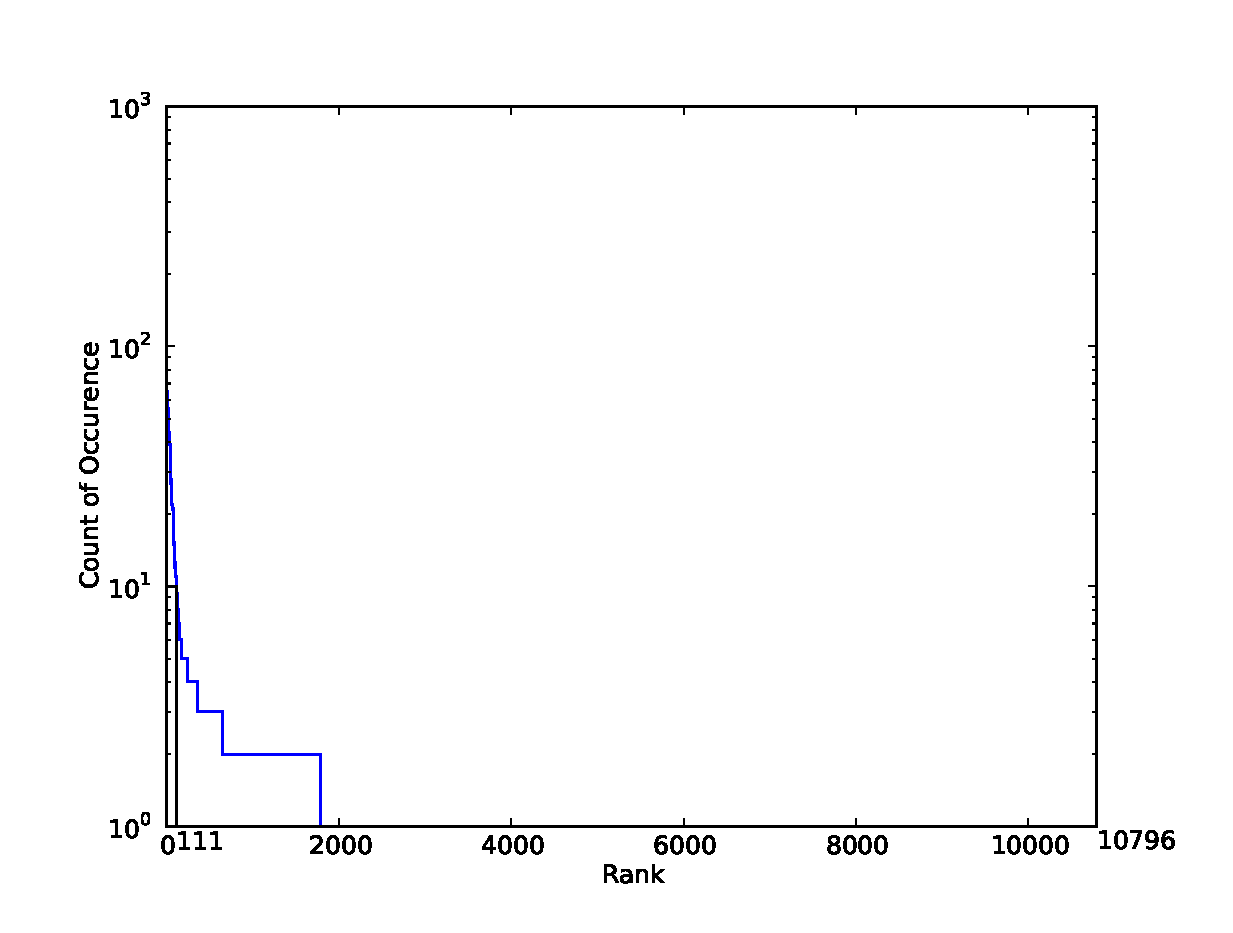
\epsfig{file=happy_sample_size_2.eps, width=0.55\textwidth}\\
    Buddha\\
    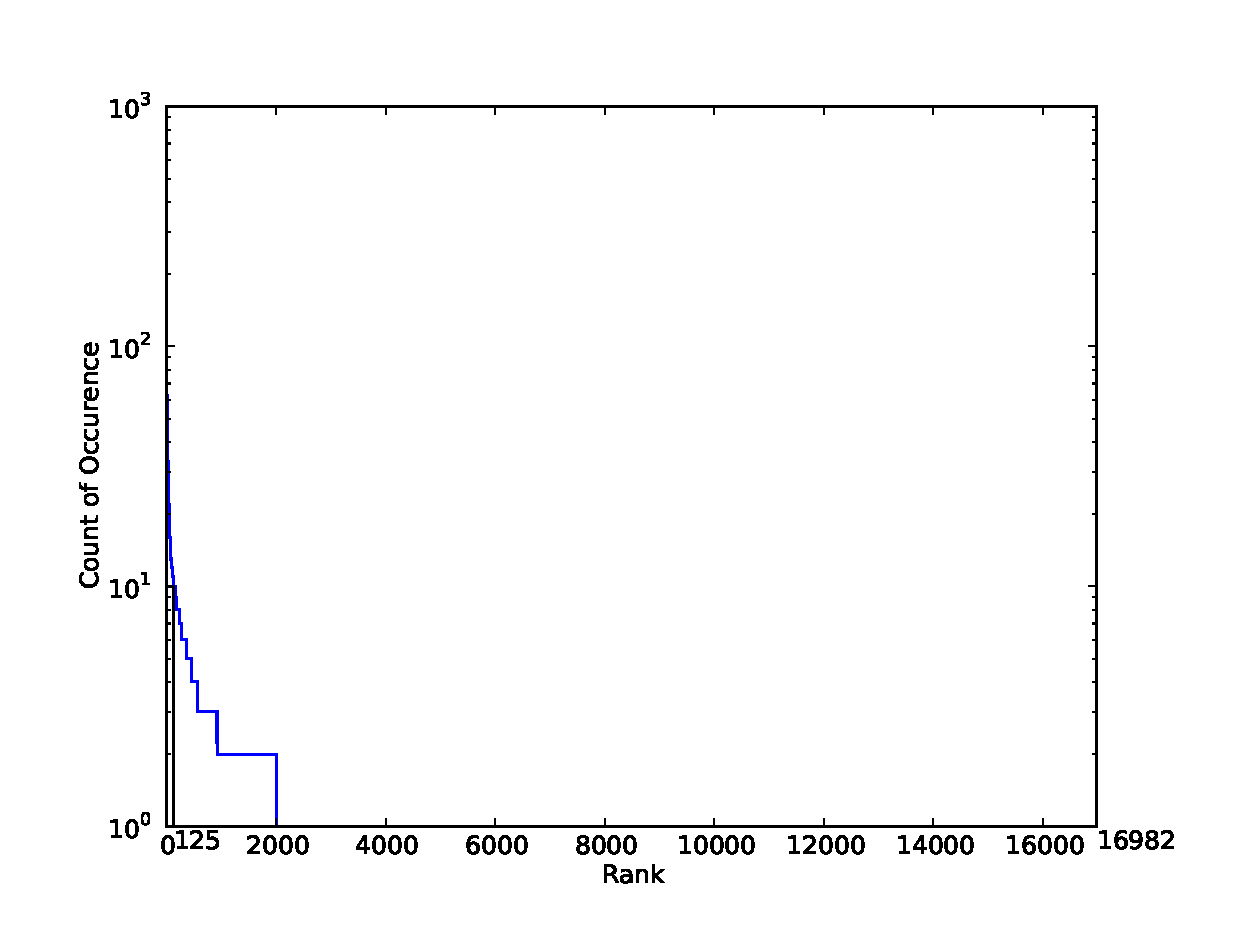
\epsfig{file=dragon_sample_size_2.eps, width=0.55\textwidth}\\
    Dragon\\
    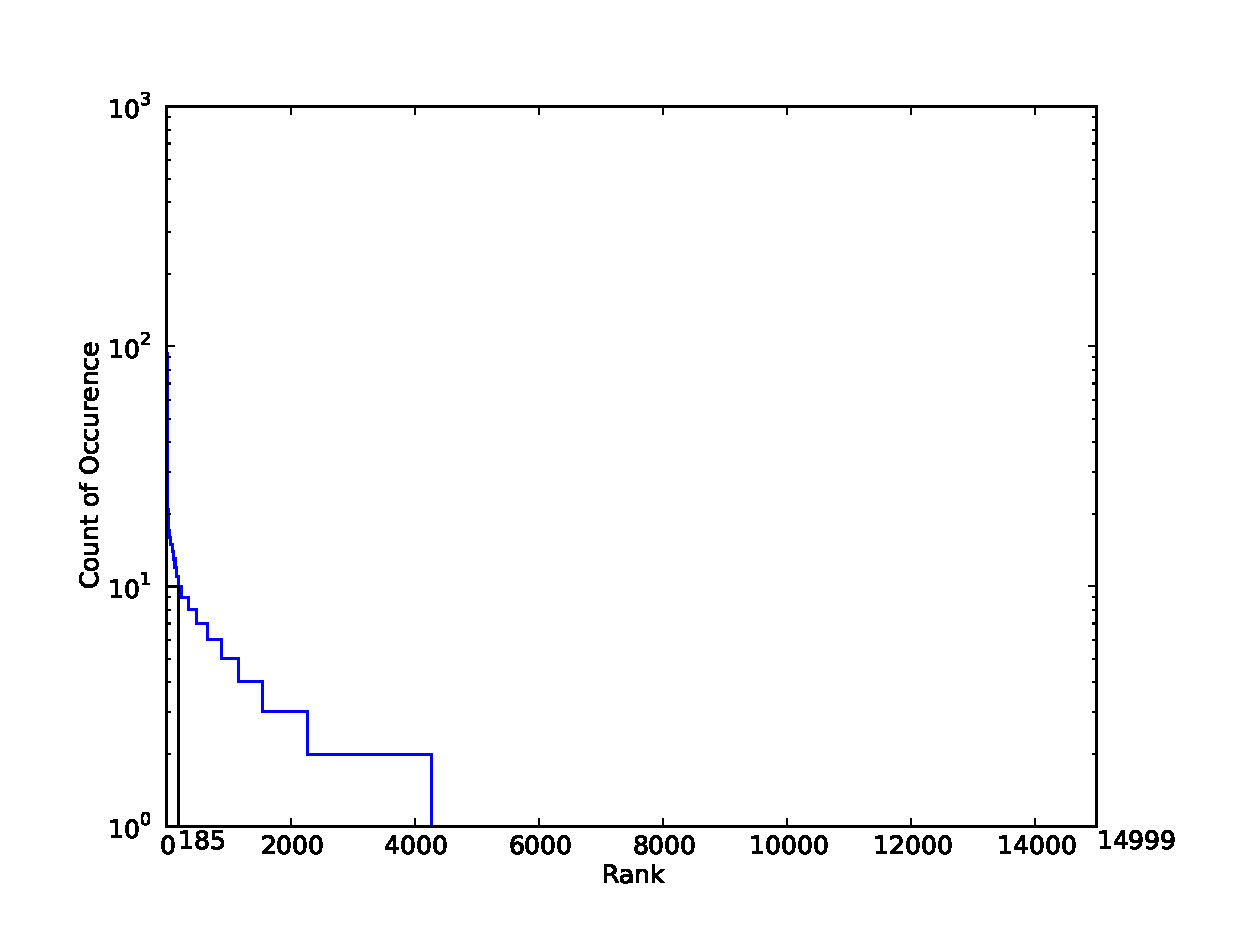
\epsfig{file=thai_sample_size_2.eps, width=0.55\textwidth}\\
    Thai Statue
    \caption{The number of samples on all combinations of viewpoint and previous action, and the combinations are sorted from the most popular to the least popular.}
    \label{f:user:sample_size_2}
\end{figure}
We ignore those combinations with  less than 10 samples.
The accuracy of this method can be seen in Figure \ref{f:user:accuracy_comp}.
This method has the highest accuracy among the four methods.

We compare the four methods in Figure \ref{f:user:accuracy_comp} for three meshes\footnote{
To increase the sample size, we aggregate the data of the three version of the same mesh together.
It is reasonable because the meshes has a defect are almost identical to the original one, 
and users do not know which one has defect in advance. Therefore, their behavior are similar to
all three versions of the same mesh.}.
Our conclusion is that the user action is somewhat predictable and the prediction is simple.
We can always predict the next action same as the previous one without considering
any extra information, and the accuracy is good enough. 
Considering both previous action and viewpoint has the highest accuracy,
but it depends on the statistics of user behavior and differs on every mesh. Hence, it can only 
be done when enough user traces are already collected for a specific mesh. 
The slightly better accuracy may not justify the much higher complexity.
\begin{figure}
    \centering
    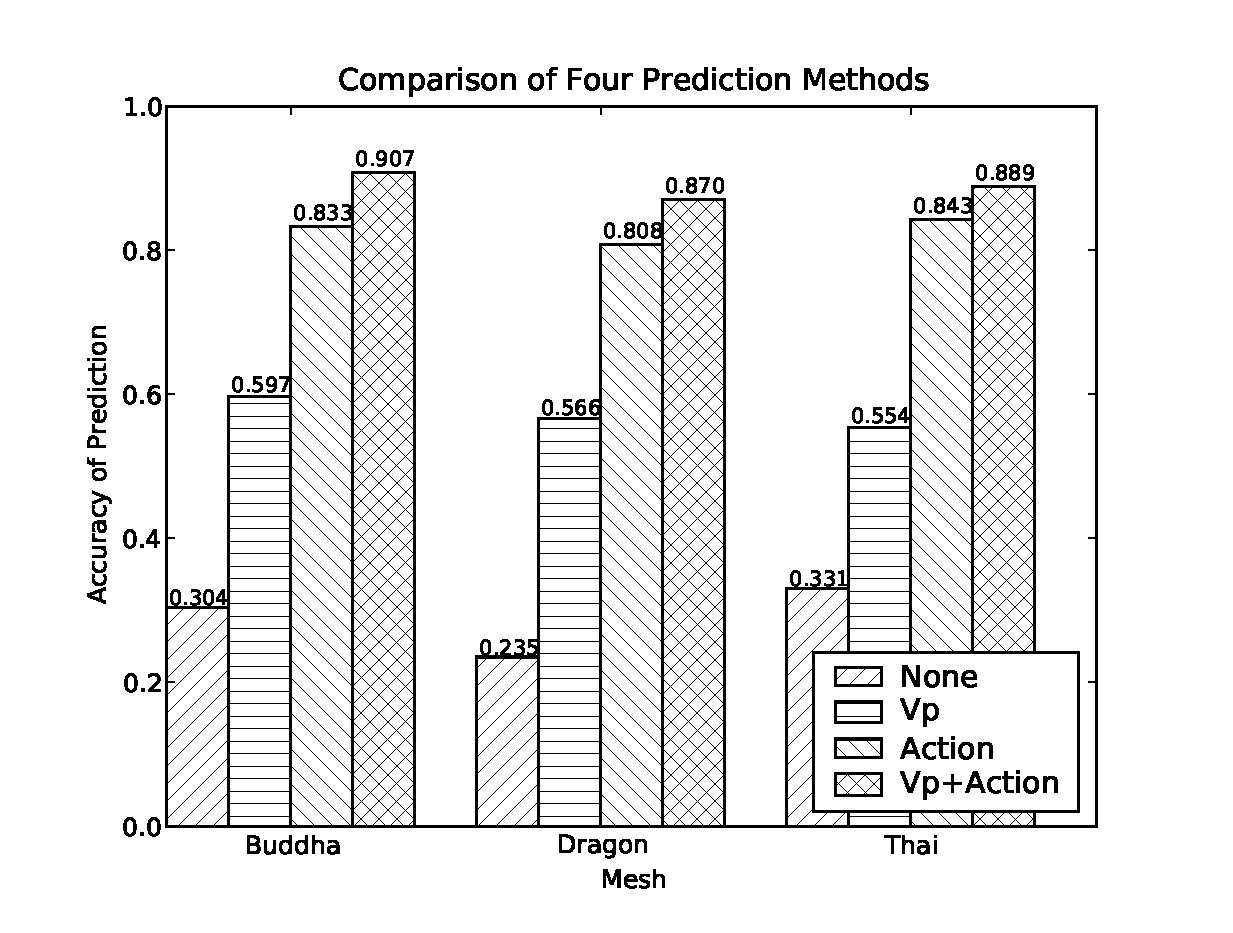
\epsfig{file=accuracy_comp.eps, width=0.65\textwidth}
    \caption{The accuracy of four prediction methods.}
    \label{f:user:accuracy_comp}
\end{figure}

\section{Generating Synthetic Traces}
To evaluate the effectiveness and performance of a system, we often need many user traces. 
It is expensive to collect a large number of real traces. 
A cheaper way is to consider a user trace as a Markov chain
and derive the transition matrix from the collected traces.
Then following the transition matrix, we can generate as many traces as we want.

The viewpoint, represented as a 6-tuple: {$x, y, z, \theta_x, ay, \theta_z$}
as introduced in Section \ref{s:user:study}, can be defined as the states in the Markov chain.
According to the observation that the previous actions highly affects the next action
(Section \ref{ss:user:predictability}),
it is not a first order Markov chain because
the previous states affect the transition probability. 
It, however, is not practical to consider the whole history before. 
To make the analysis possible, we consider only one step before and assume
``(previous state, current state)'' decides ``next state''. In other words, 
it is a second order Markov chain. 
As we introduced in Section \ref{ss:user:predictability}, the latest action affects the most, so
this simplification is reasonable.

We can reduce the second order Markov chain to first order by defining the current state as
(previous viewpoint, current viewpoint). After a user action, the new state becomes 
(current viewpoint, next viewpoint) (See Figure \ref{f:user:reduction}(A)). 
Then, the transition probability only depends on the current state.
Notice that (previous viewpoint, current viewpoint) is equivalent to (current viewpoint, previous action), 
so we finally define the state to be ($x, y, z, \theta_x, \theta_y, \theta_z, A_p$). 
(See Figure \ref{f:user:reduction}(B)).
\begin{figure}
    \centering
    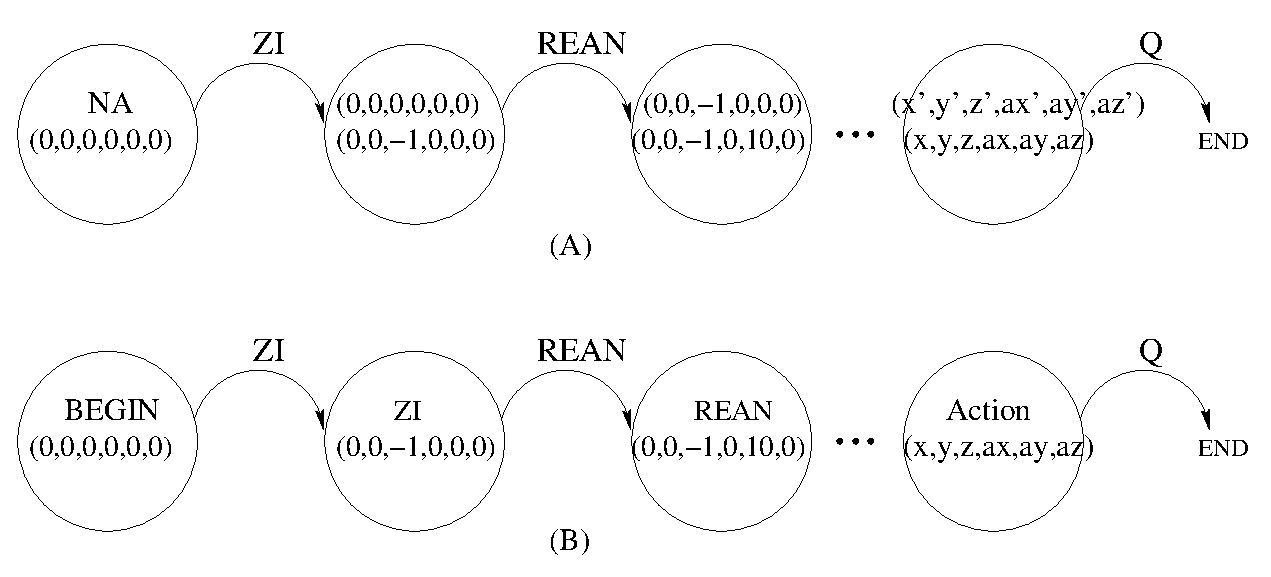
\epsfig{file=reduction.eps, width=0.6\textwidth}
    \caption{(a), State = (previous viewpoint, current viewpoint); (b), State = ($x, y, z, \theta_x, \theta_y, \theta_z, A_p$)}
    \label{f:user:reduction}
\end{figure}

Each record in the user traces can be seen as a sample of this random process.
From these samples, we can compute the transition probability between two states, and hence
the transition matrix, with which we can generate synthetic traces.

This method, however, has limitations when the number of collected traces is small. First, if a viewpoint is 
never accessed by the real traces, it will not accessed by synthetic traces either. Therefore, no matter how
many synthetic traces are generated, the number of accessed viewpoints is upper-bounded. 
Second, due to the large sample space and limited number of samples, most of the states has only one sample
(See Figure \ref{f:user:sample_size_2}). 
In other words, in the transition matrix, the next action for most states are determined. 
As a result, after several steps, the synthetic trace follows the exact path as one of the real traces. Therefore, the synthetic traces are not random enough.

To address these two limitations, we propose a method to generate traces that are more random in the next section.
It is based on a simplified model, which does not directly derive and follow the transition matrix.

\subsection{Simplified Model}
To generate a synthetic trace, we need to determine the probability of each possible $A_n$ based on current
state ``($x,y,z,\theta_x,\theta_y,\theta_z,A_p$)''. Due to the limited number of samples, we cannot obtain the reliable
transition probability for most of the states. As a result, we need to find a new way to determine the 
conditional distribution of $A_n$.

To address the problem of lacking samples, we consider only the main factors 
affecting the probability of $A_n$ and ignore others. 
According to our observation, 
repeating the previous action has the highest probability in most cases. 
Therefore, the previous action is chosen as one of the most important factor. 
Based on the relation with the previous action, we categorized actions to three groups: 
\textit{repeat}, \textit{reverse}, and \textit{change}. 
We determine the next action in two steps:
\begin{enumerate}
    \item We determine the probability of ``repeat'', ``reverse'', and ``change'',
        i.e. $Pr(repeat|_{\textrm{current state}})$, 
        $Pr(reverse|_{\textrm{current state}}$, 
        and $Pr(change|_{\textrm{current state}})$,
        respectively. 
    \item We decide the distribution of $A_n$ if ``change'' is decided, 
        i.e. $Pr(A_n |_{\textrm{current state}, A_n != A_p, A_n != \textrm{reverse}(A_p)})$ 
        for each possible $A_n$. 
\end{enumerate}


%We think it is mainly because users tend to press the same key multiple times. 
%Sometimes, when users moves the mesh to the edge, they tend to reverse the action to move it back. 
%Otherwise, if the user has decided to change to a new direction, 
%then the previous action may have no effect on the next action.

%We assume that only step 1 depends on the previous action, and step 2
%only depends on ($x,y,z,\theta_x,\theta_y,\theta_z$). 

In step 1, besides this most important factor, the previous action, we consider only one coordinate instead of six.
%In step 1, the repeat probability depends on the previous action and the 6-tuple ($x, y, z, \theta_x, \theta_y, \theta_z$).
%To simplify the model, we only consider the most important factor and ignore others. 
As we know, an action only changes one coordinate in the 6-tuple. We call this coordinate \textit{corresponding coordinate}.
For example, the corresponding coordinate of ``Move Left'' is $x$, and the corresponding coordinate of 
``Revolving Clockwise'' is $\theta_y$. 
When users are repeating or reversing the previous action, 
only the corresponding coordinate is changed. 
As a result, we only consider the corresponding coordinate in determining the repeat probability. 
For example, when a user keeps pressing ``Move Left'', the mesh may nearly be out of the viewable area, 
then the probability of ``repeat'' decreases, and the probability of ``reverse'' increases. 
Another example is that when the user keeps pressing ``Revolve Clockwise'' and find something interesting
in the mesh from the current direction,
the probability of ``repeat'' decreases and the probability of ``change'' increases.
In summary, in this simplified model, we assume that the probability of ``repeat'', ``reverse'', and ``change''
only depends on ``(previous action, corresponding coordinate)''.
As a result, the number of available samples of each combination increases a lot compared with the first method
(See Figure \ref{f:user:newsample}). 
\begin{figure}
    \centering
    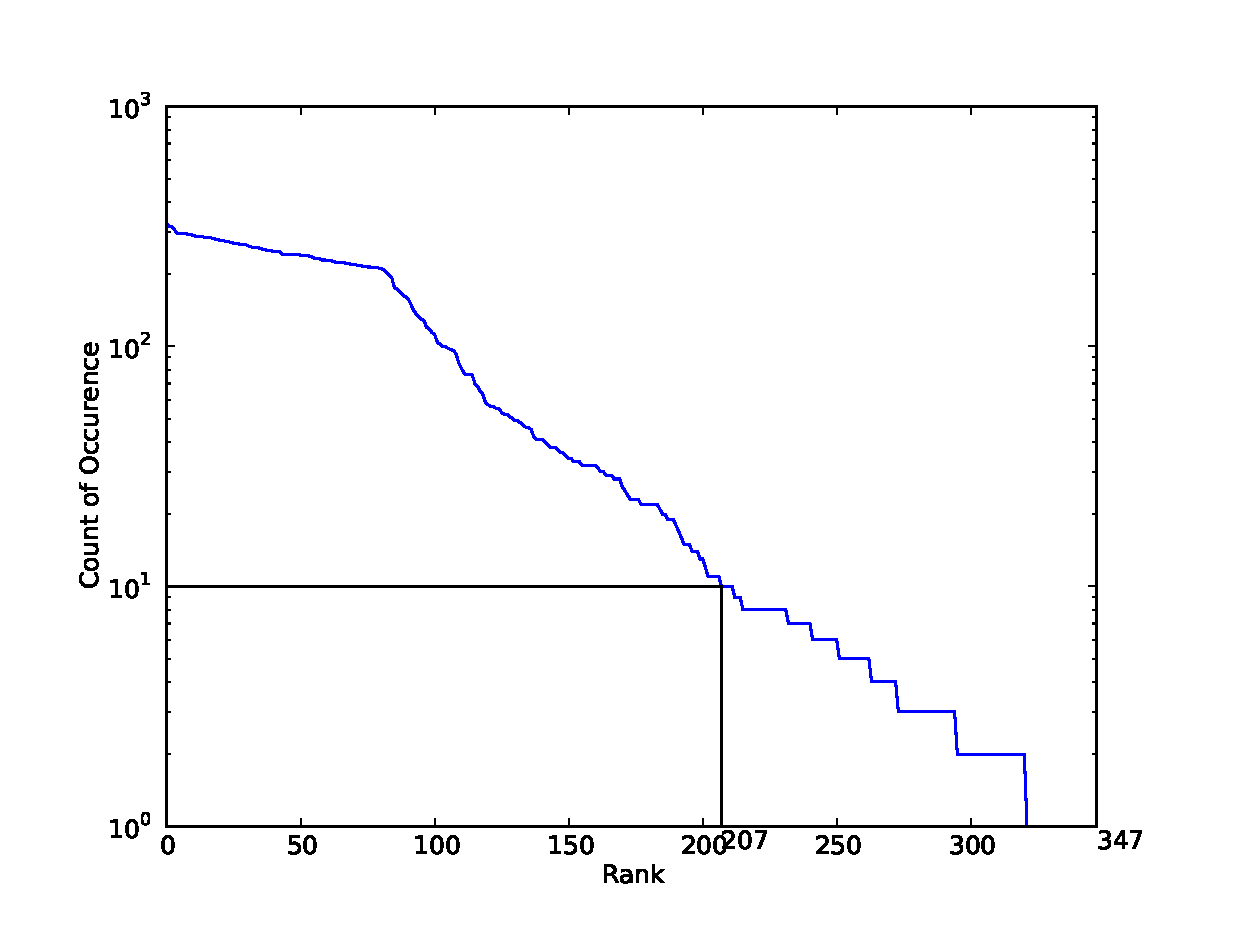
\epsfig{file=new_sample.eps, width=0.5\textwidth}
    \caption{The sample size of each combination (previous action, corresponding axis), 
    sorted from the most popular to least popular.  Mesh: Thai}
    \label{f:user:newsample}
\end{figure}

In step 2, we need to determine $Pr(A_n |_{\textrm{current state}, A_n != A_p, An != \textrm{reverse}(A_p)})$
for each possible $A_n$. In this step, we ignore the effect of previous action. 
We think the high probability of ``repeat'' is mainly because users tend to press the same key multiple times. 
It affects the probability of ``change'', but its effect on which action to choose as ``change'' is little.
%When a user has decided to go along another axis, we think the previous action has little effect on the choice of
%next action. 
Hence, we assume that $Pr(A_n |_{\textrm{current state}, A_n != A_p, An != \textrm{reverse}(A_p)})$
only depends on $(x, y, z, \theta_x, \theta_y, \theta_z)$. Here, all coordinates, except the corresponding coordinate
(it will not be changed since ``repeat'' and ``reverse'' are already excluded from the choices),
are important to decide the next action, so the sample size is not large enough to derive the probabilities
from the trace.
Instead, we propose a heuristic based on the assumption
\[
    Pr(x, y, z, \theta_x, \theta_y, \theta_z) = Pr(x)Pr(y)Pr(z)Pr(\theta_x)Pr(\theta_y)Pr(\theta_z)
\]
In other words, we assume that the probability for a viewpoint has a specific coordinate is independent with its 
other coordinates. This is an assumption to simplify our model, and will introduce some difference between
synthetic traces and real traces. In the validation part, however, we show that the difference is not 
significant.

At a specific viewpoint $Vp$: $(x, y, z, \theta_x, \theta_y, \theta_z)$, if we change the value of $x$, 
then we stay in the 5-dimension space
\[
    (Y=y, Z=z, AX=\theta_x, AY=\theta_y, AZ=\theta_z).
\]
The probability of the viewpoint staying in this space is 
\begin{align*}
    &Pr(y, z, \theta_x, \theta_y, \theta_z)\\
    =&Pr(y)Pr(z)Pr(\theta_x)Pr(\theta_y)Pr(\theta_z)\\
    =&\frac{Pr(x)Pr(y)Pr(z)Pr(\theta_x)Pr(\theta_y)Pr(\theta_z)}{Pr(x)}\\
    =&\frac{Pr(x, y, z, \theta_x, \theta_y, \theta_z)}{Pr(x)}\\
    =&\frac{Pr(Vp)}{Pr(x)}.
\end{align*}
Similarly, we can know the probability of the viewpoint staying in other spaces. 

Hence, we set the probability of changing a value of a axis to be proportional to the probability of staying in the
corresponding space. For example, the probability of changing $x$ when the previous action is on $AY$
\begin{align*}
    =&\frac{\frac{Pr(vp)}{Pr(x)}}
            {\frac{Pr(vp)}{Pr(x)}
            +\frac{Pr(vp)}{Pr(y)}
            +\frac{Pr(vp}{Pr(z)}
            +\frac{Pr(vp)}{Pr(\theta_x)}
            +\frac{Pr(vp)}{Pr(\theta_z)}}\\
    =& \frac{\frac{1}{Pr(x)}}
            {\frac{1}{Pr(x)}
            +\frac{1}{Pr(y)}
            +\frac{1}{Pr(z)}
            +\frac{1}{Pr(\theta_x)}
            +\frac{1}{Pr(\theta_z)}
            }.
\end{align*}
Similarly, we can know the probability of changing other coordinates. Intuitively, we can think $Pr(x)$ as 
the popularity of current $x$ value. The above equation means that we tends to change the coordinate having low
popularity.

%We verify it with the traces we obtained and we can find that it is a reasonable simplification
%except for the first several viewpoints. 
%These first several viewpoints are the default viewpoint and its neighbors almost all users will pass, 
%so their probability is significantly higher. We ignore these points in this simplified method.
%Because we have enough samples for these viewpoints, we
%still use the standard method to derive the transition probability for these viewpoints. 

Next, for each axis we have two directions to move, and we need to know the probability of each direction.
We assume users tend to move to a position with higher popularity, i.e. $Pr[vp]$. We set the probability 
of a direction to be proportional to the sum of popularity of its several neighbors in that direction (we choose
3 neighbors in our implementation). 
For example, if the axis to change is $X$ and its current value is $x$, 
the probability of moving to $x+1$  
\begin{align*}
   =&\frac{Pr(x+1)+Pr(x+2)+Pr(x+3)}
          {Pr(x+1)+Pr(x+2)+Pr(x+3)+Pr(x-1)+Pr(x-2)+Pr(x-3)}.
\end{align*}
Notice all these viewpoints have same $y$, $z$, $\theta_x$, $\theta_y$, and $\theta_z$.
We consider several neighbors instead of one because users tend to repeat 
the same action several times. 

In brief, we generate a synthetic trace as follows:
\begin{enumerate}
    \item Determine the session time according to the distribution of session time we derived from the real traces.
    \item For the default viewpoint, we derive the transition probability from the traces and decide the
        next action based on it.
    \item For other viewpoints, we choose ``repeat'', ``reverse'', or ``change'' 
        based on {previous action, corresponding coordinate}.
    \item If we choose ``change'', 
        we first determine the axis to change based on $Pr(x)$, $Pr(y)$, $Pr(z)$, 
        $Pr(\theta_x)$, $Pr(\theta_y)$, and $Pr(\theta_z)$. 
        Next, we choose the direction based on the popularity of three
        neighbors in both directions.
    \item We randomly select a think time from two different distributions 
        based whether the action is ``repeat'' or not (see Section \ref{ss:user:thinktime}).
        Then go back to step 3 unless the session time is expired.
\end{enumerate}

The synthetic traces generated by our method satisfying some important requirements. 
When replaying the traces we generated, the mesh will not stay in abnormal state for long 
(abnormal positions include upside down, titled, out of viewable area, etc.).
Since we decide the ``repeat'' and ``reverse'' probability considering the corresponding coordinate,
the probability for the mesh to enter abnormal state is low, and it tends to go back to normal state
by ``reverse'' action. 
Moreover, whenever ``change'' is chosen, 
the mesh tends to go to a more normal state (a state having higher probability). 

\subsection{Validation}
In this section, we validate our model by comparing the synthetic traces we generated with the real traces.
We generated 10000 synthetic traces following the simplified model we introduced in the last section.
Thai mesh is chosen as the mesh used in this validation because of its high complexity and hence
the high challenge.

First, we compare the unconditional probability of each action in the traces. 
From Figure \ref{f:user:frequency_comp}, we can see that the traces we generated fit well with the real traces. 
This result is impressing because we never consider unconditional probability in our model, but  
still the traces generated have similar unconditional probability for each action.
\begin{figure}[htdp!]
    \centering
    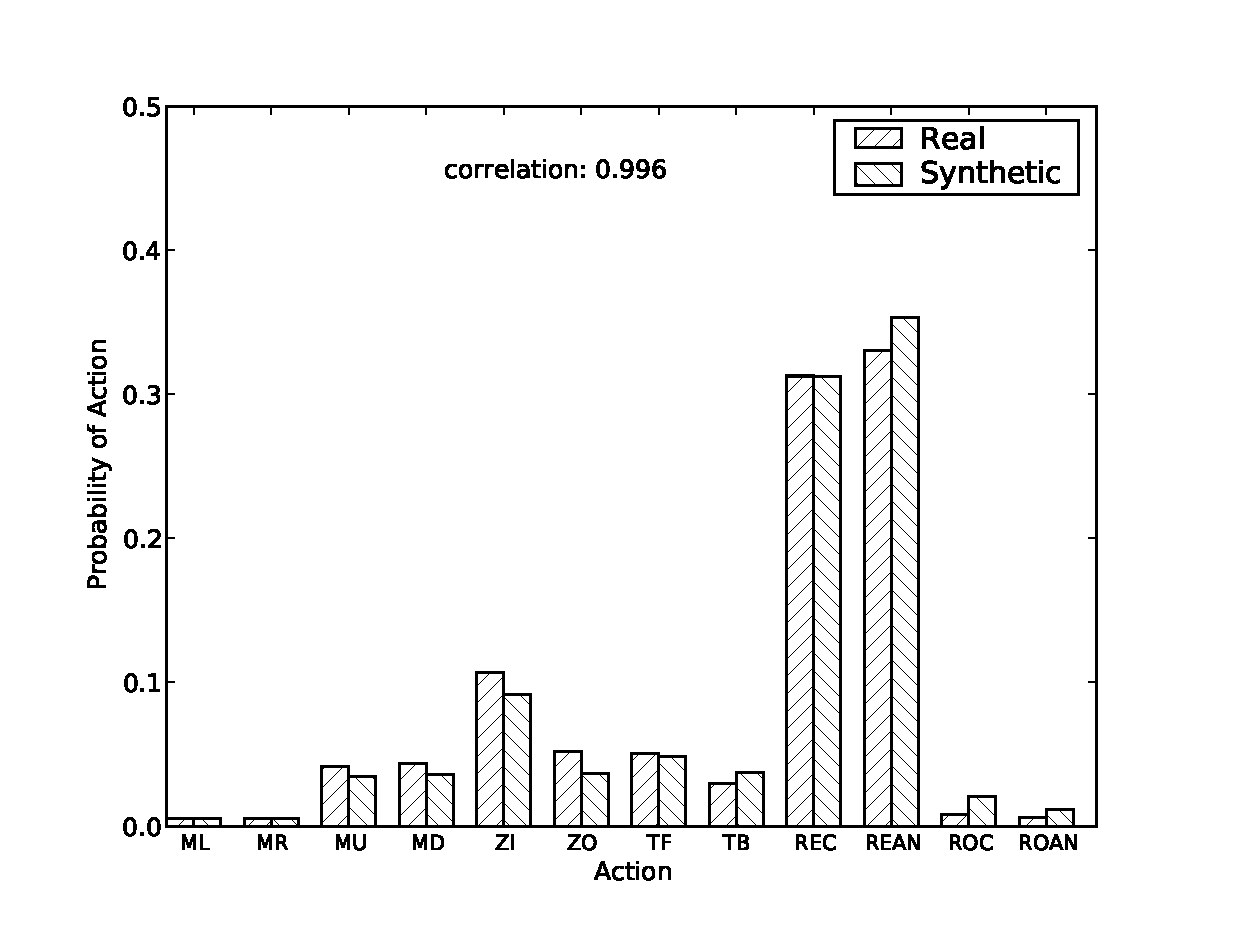
\epsfig{file=general_prob_comp.eps, width=0.5\textwidth}
    \caption{Comparison of occurrence frequency of each action.}
    \label{f:user:frequency_comp}
\end{figure}

Second, we compare the probability of repeating the previous action, including unconditional repeat probability
and the repeat probability under different previous action. We can see from Figure \ref{f:user:repeat_prob_comp},
the synthetic traces we generated has similar repeating probability under all conditions.
\begin{figure}[htdp!]
    \centering
    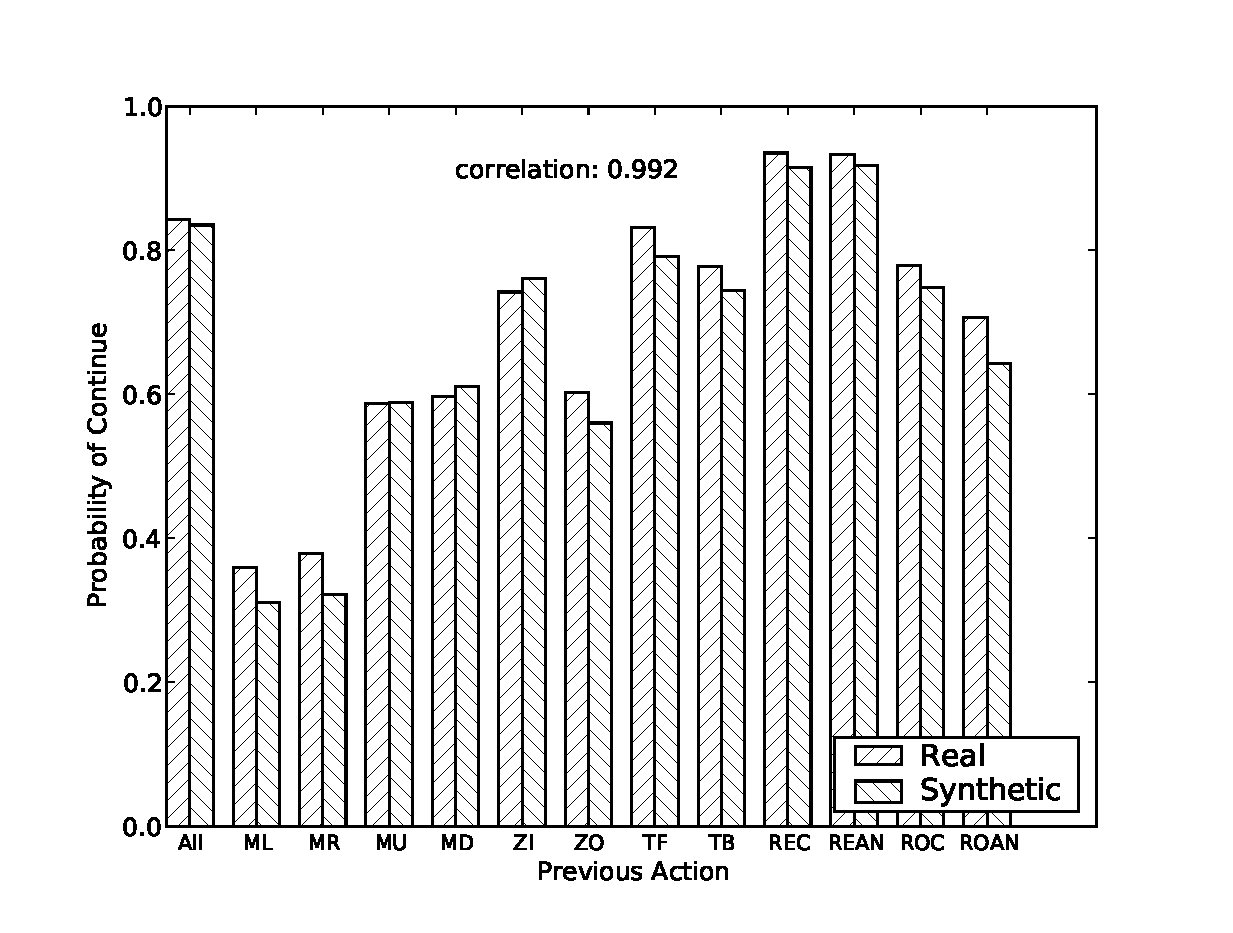
\epsfig{file=repeat_prob_comp.eps, width=0.5\textwidth}
    \caption{Comparison of unconditional repeat probability and repeat probability under different previous actions.}
    \label{f:user:repeat_prob_comp}
\end{figure}

Third, we compare how the viewpoints distributed on each axis, 
i.e. the value of $Pr(x)$, $Pr(y)$, $Pr(z)$, $Pr(\theta_x)$, $Pr(\theta_y)$, and $Pr(\theta_z)$. 
Figure \ref{f:user:axis_distribution} shows that the synthetic traces we generated has similar distributions on all 
axises. Among the six axises, only the $Y$ axis has a slightly higher error. The synthetic traces tend to stay in the
center ($0$) more often. The correlation between these two set of values, however, is still close to $1$. 
Again, this result is interesting. Although we have considered these probabilities in selecting new action when
``change'' is selected, the majority of selections (recall that more than 80\% of actions are ``repeat'')
has nothing to do with these values. 
\begin{figure}[htdp!]
    \centering
    \begin{tabular}{cc}
    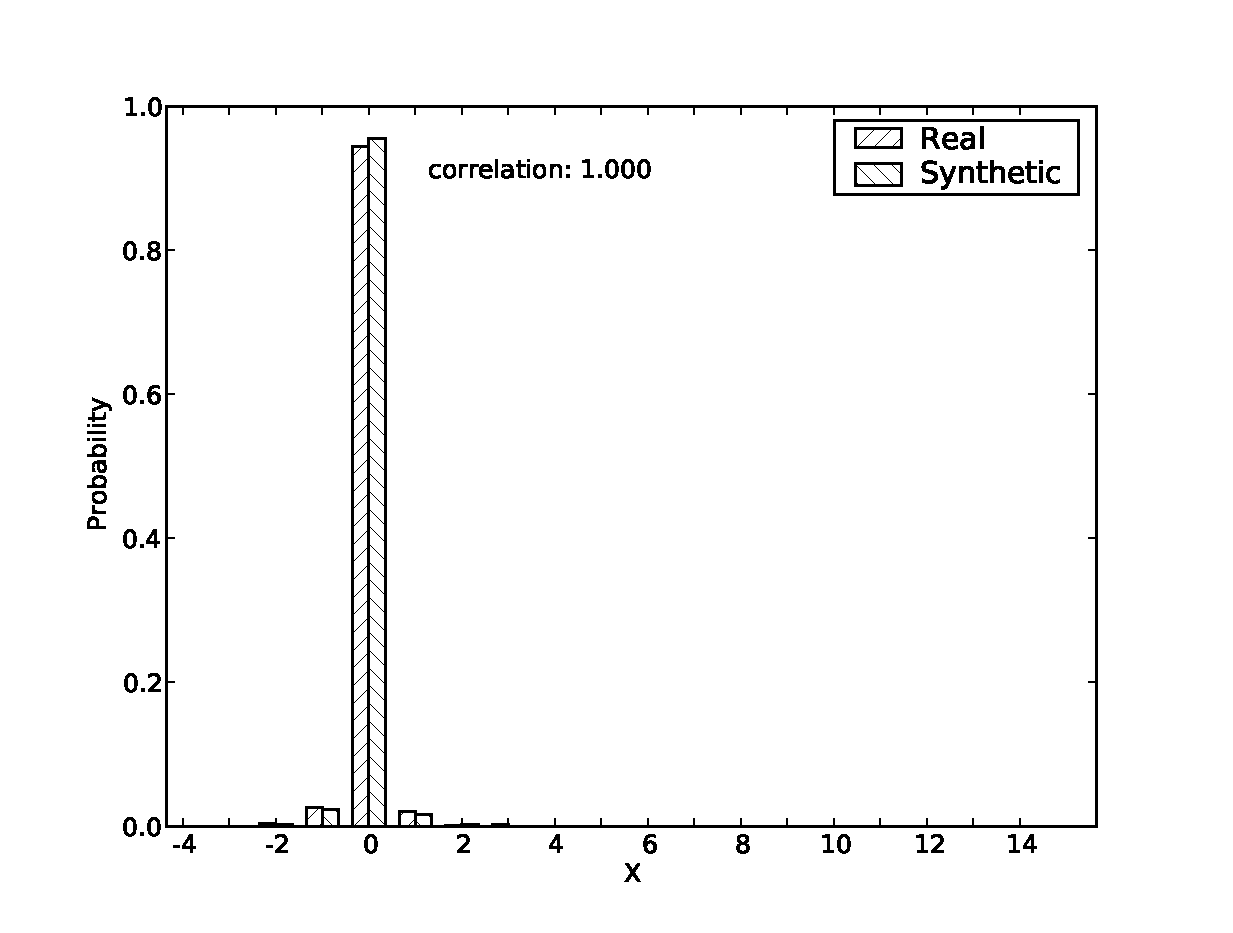
\epsfig{file=x.eps, width=0.45\textwidth}&
    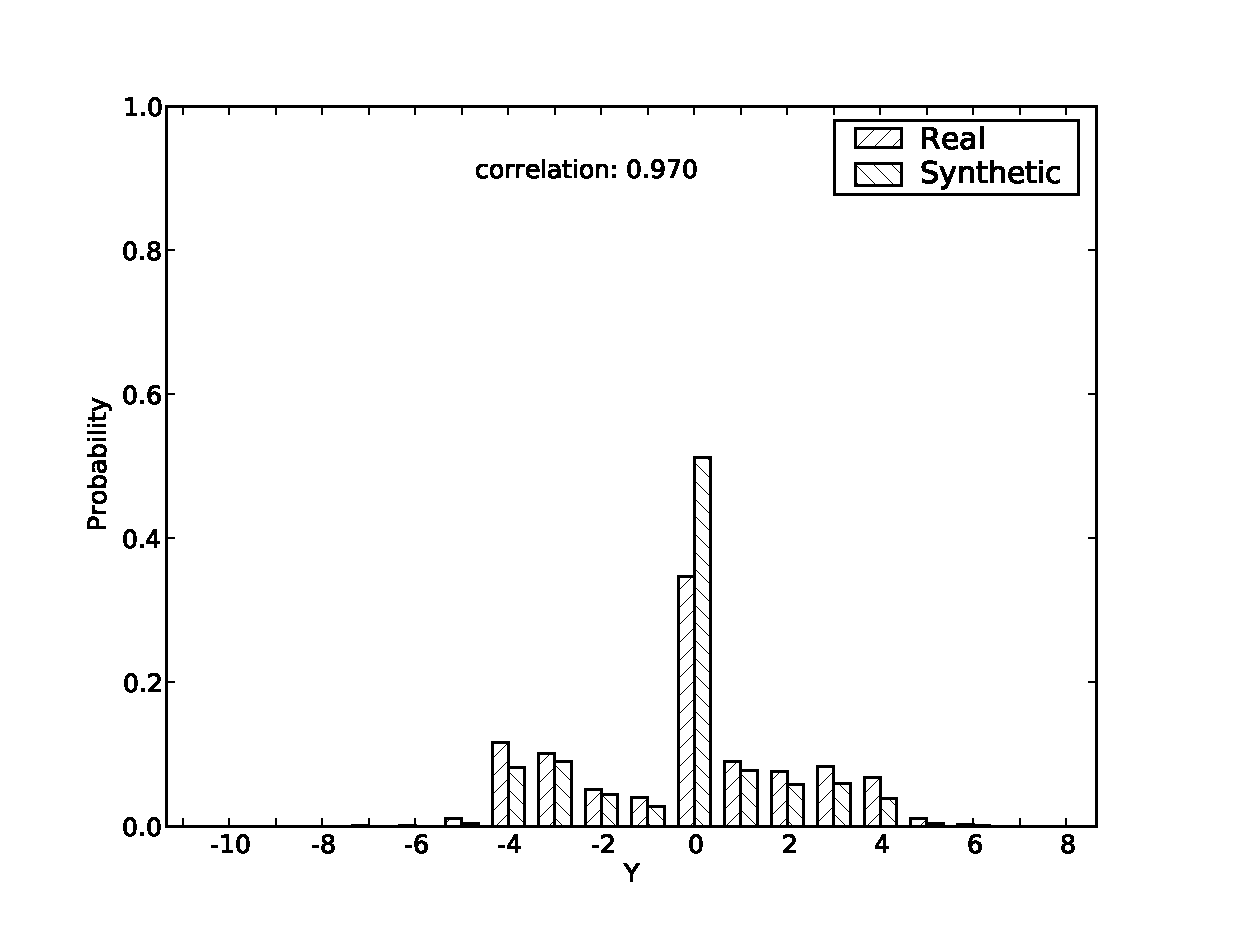
\epsfig{file=y.eps, width=0.45\textwidth}\\
    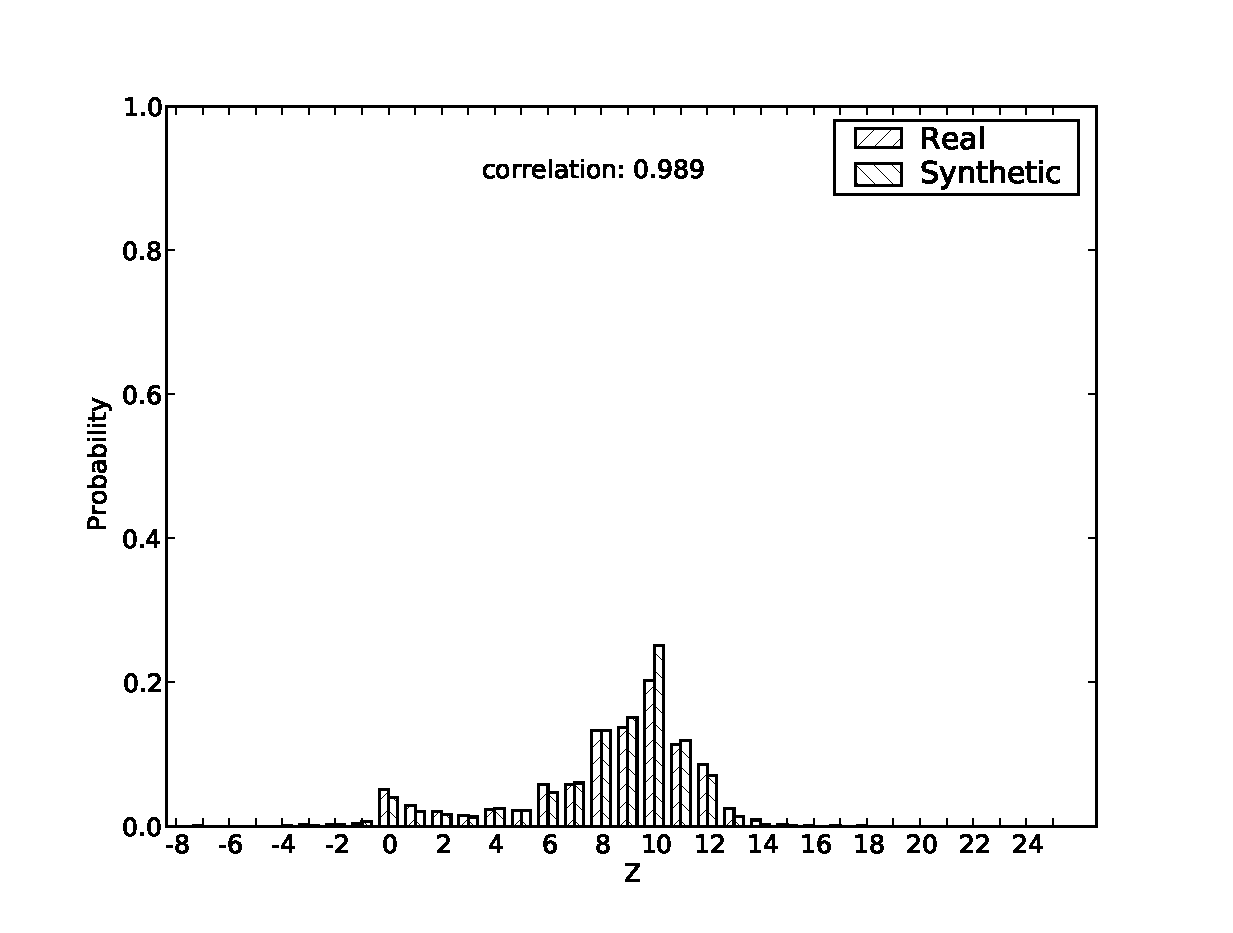
\epsfig{file=z.eps, width=0.45\textwidth}&
    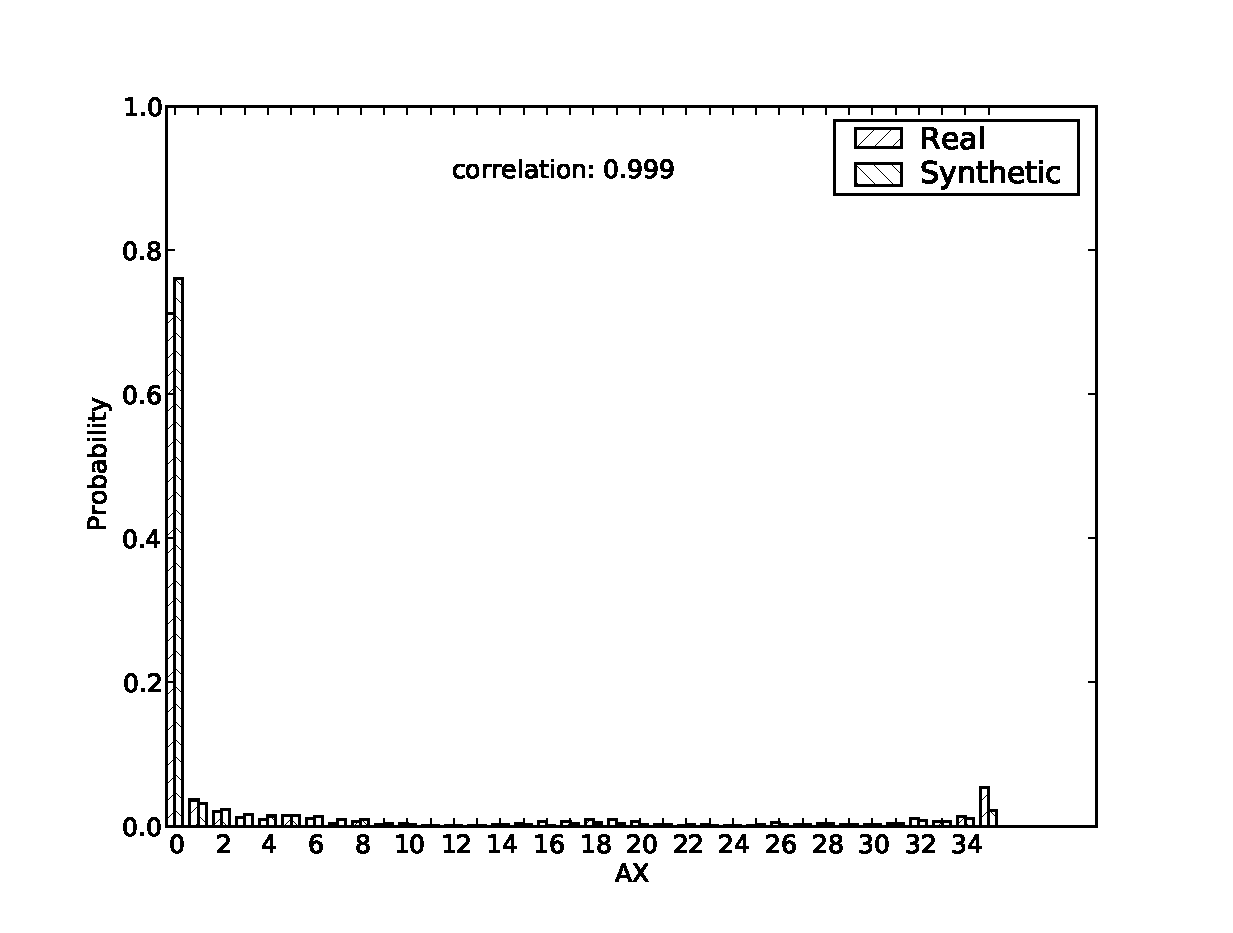
\epsfig{file=ax.eps, width=0.45\textwidth}\\
    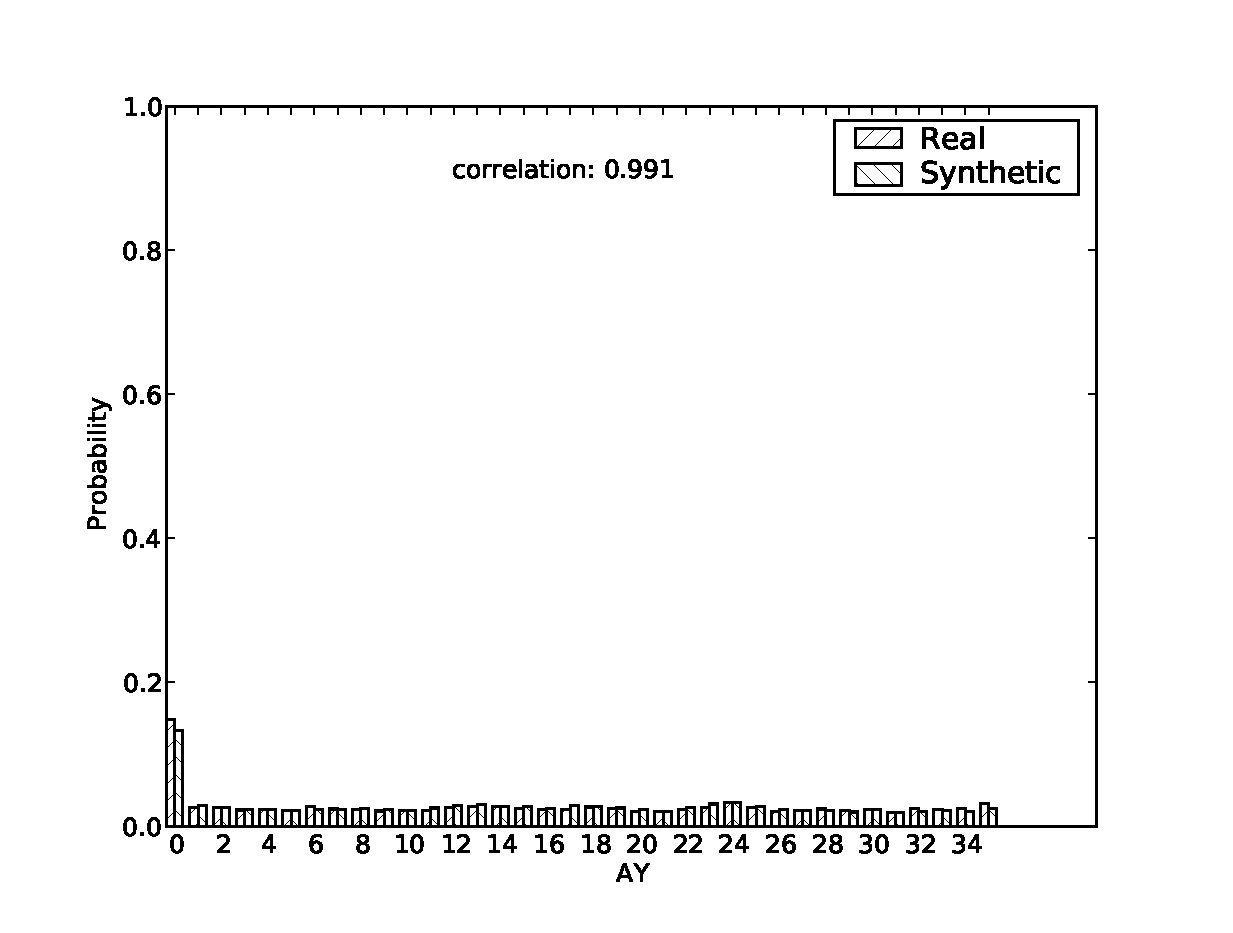
\epsfig{file=ay.eps, width=0.45\textwidth}&
    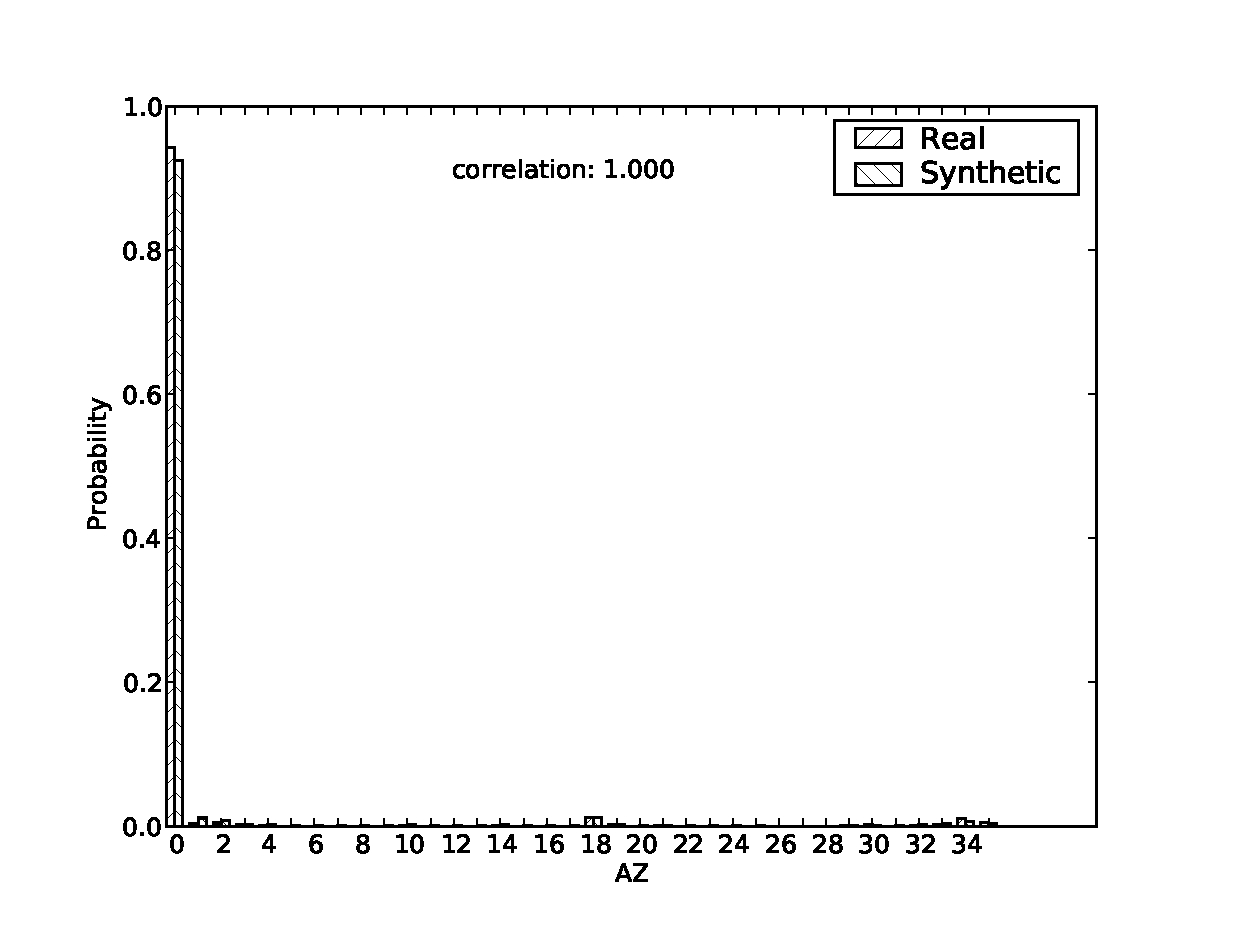
\epsfig{file=az.eps, width=0.45\textwidth}
    \end{tabular}
    \caption{Comparison of distribution of viewpoints on different axises.}
    \label{f:user:axis_distribution}
\end{figure}

The final comparison is on the transition probability on certain state, $Pr(A_n|_{(x, y, z, \theta_x, \theta_y, \theta_z, A_p)})$. 
If the Markov chain method used, the synthetic traces should have the same transition probability with the real trace.
Due to the limited sample size, however, we have to use a simplified method. 
This comparison shows how much difference we introduced by this simplification. 
We only choose some states with enough number of samples to ensure the transition probabilities
are reliable. Some of the results are shown in Figure \ref{f:user:transition_comp}.
\begin{figure}
    \centering
    \begin{tabular}{cc}
        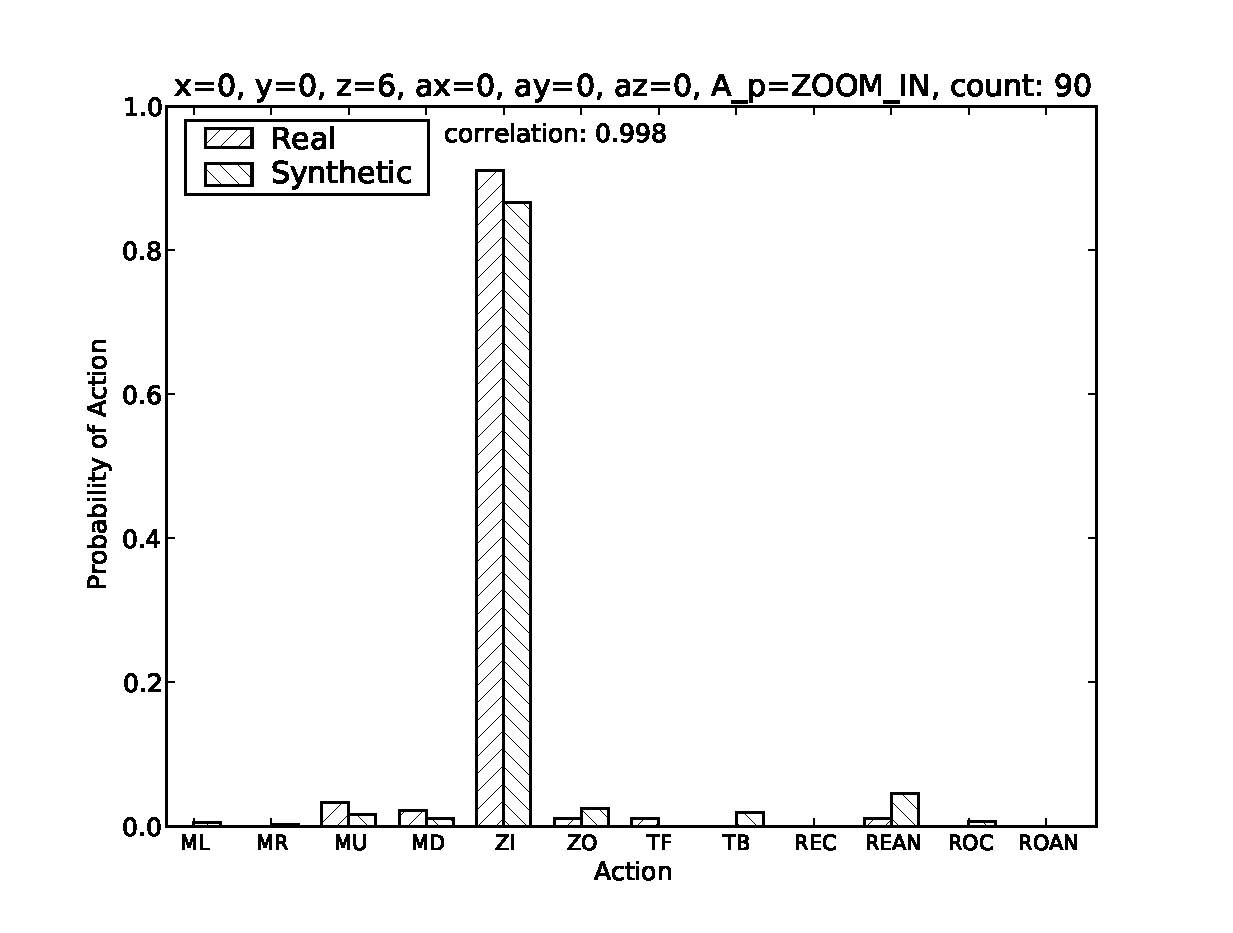
\epsfig{file=transition6.eps, width=0.45\textwidth}&
        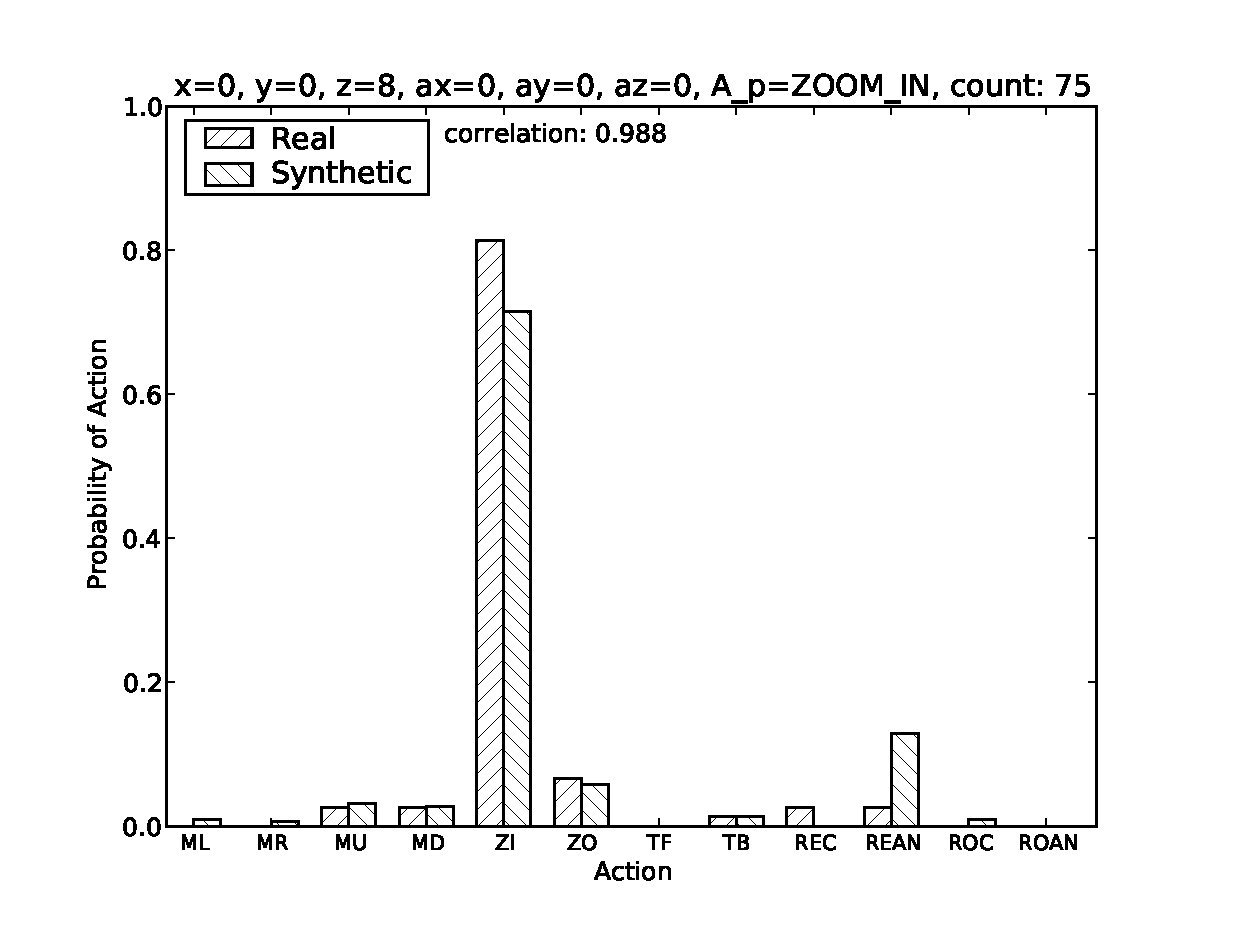
\epsfig{file=transition8.eps, width=0.45\textwidth}\\
        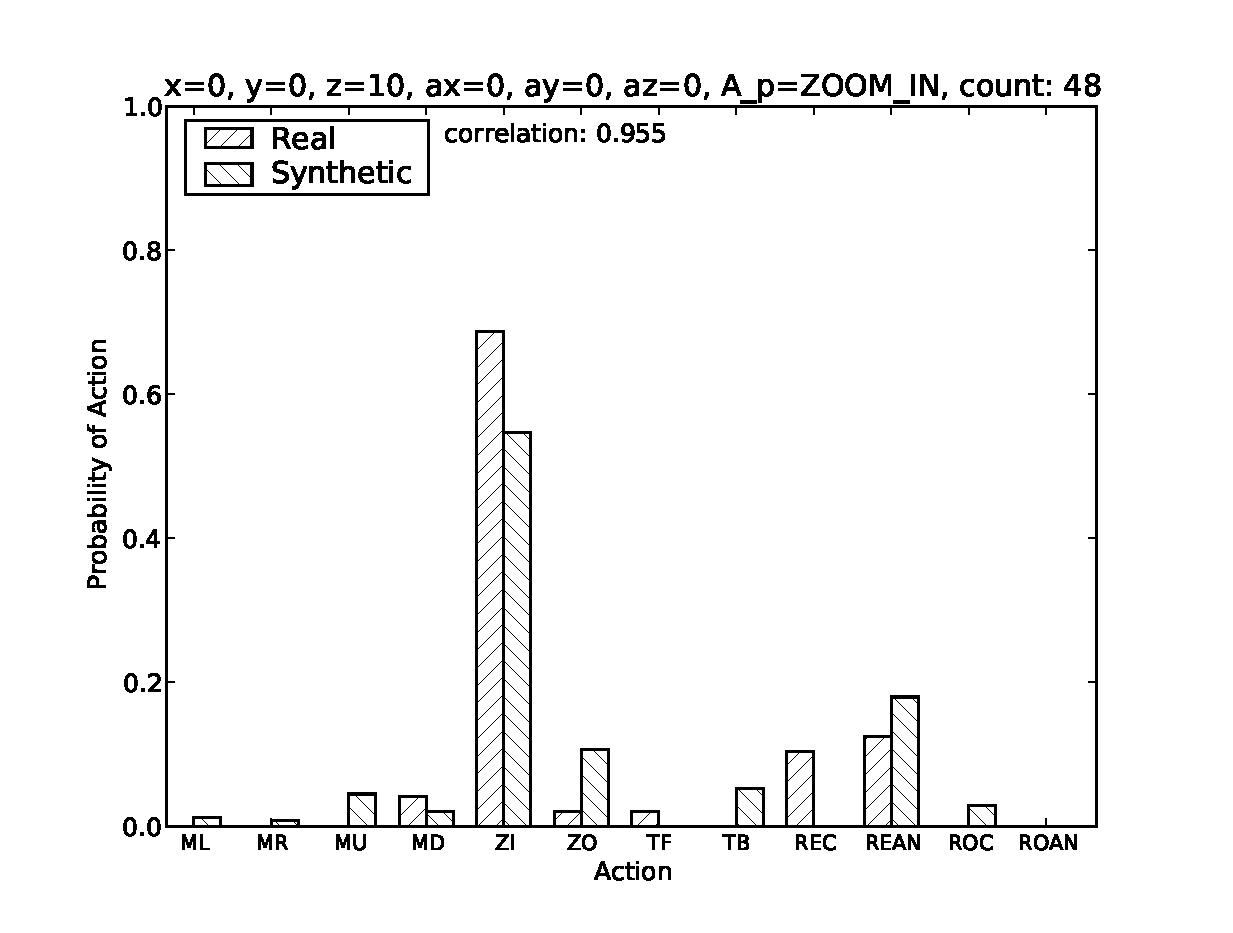
\epsfig{file=transition10.eps, width=0.45\textwidth}&
        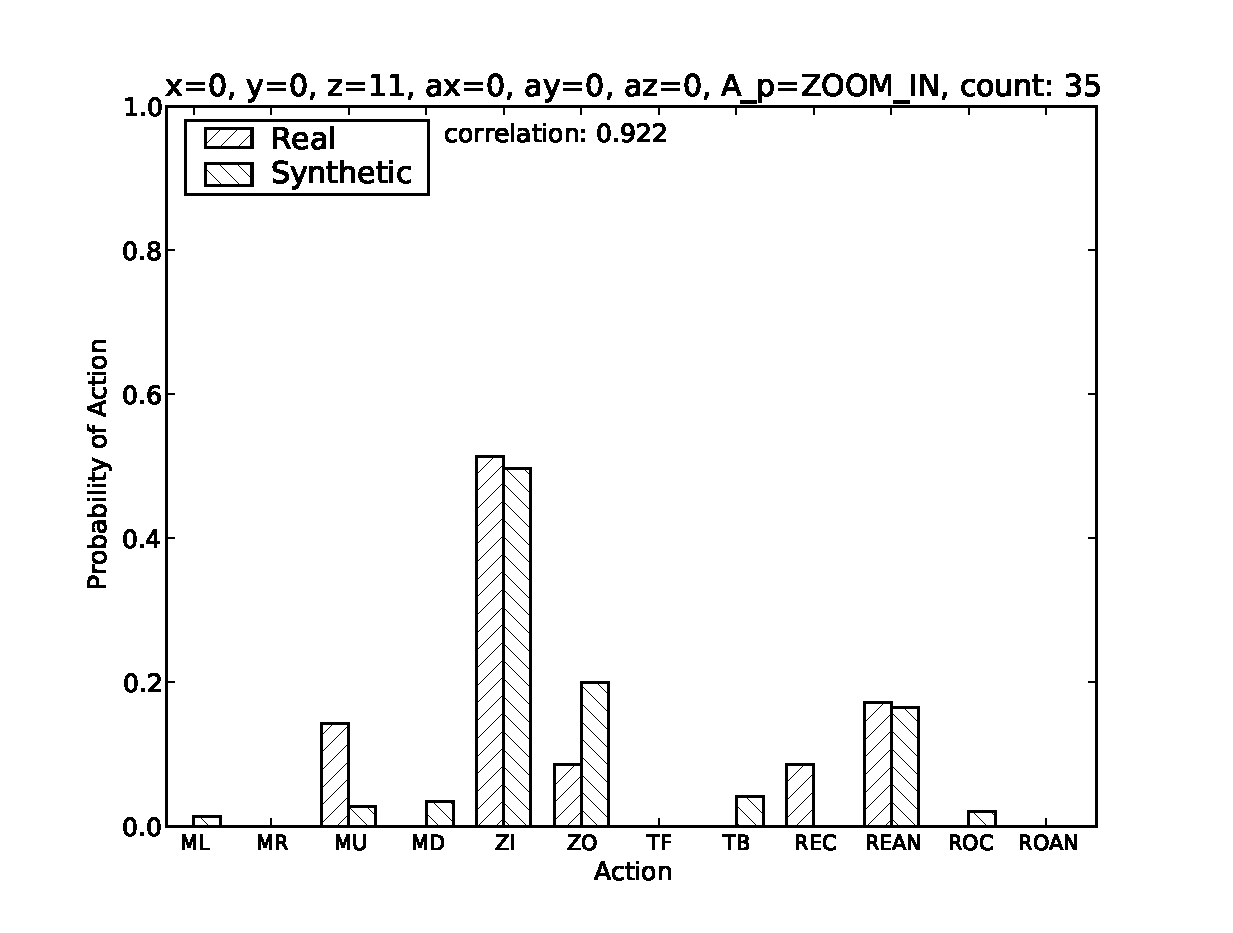
\epsfig{file=transition11.eps, width=0.45\textwidth}\\
        \epsfig{file=transition12.eps, width=0.45\textwidth}&
        \epsfig{file=transition16.eps, width=0.45\textwidth}\\
        \epsfig{file=transition17.eps, width=0.45\textwidth}&
        \epsfig{file=transition18.eps, width=0.45\textwidth}\\
    \end{tabular}
    \caption{Comparison of transition probabilities on certain states.}
    \label{f:user:transition_comp}
\end{figure}
In most of the cases, the synthetic traces have similar transition probability. The largest error happens
when the sample size is small (22) and the distribution of next action is relatively even (the 6th figure). 
In this case, the transition probability derived from the real traces itself is not so reliable. In short, due to the limited number
of real traces, the value of comparison based on states is limited. According to the results we have, however, we still can conclude 
the simplified model works well.

\section{Conclusion}
We conclude this chapter by showing the most significant findings we have.
First, the analysis of user traces reveals that locality exists in both data and viewpoint access. 
We can exploit this locality in designing progressive mesh streaming systems and rending systems.
%storing the most popular mesh data in caching proxies, the server overhead could be significantly reduced. 
Second, user actions are predictable to certain extent. The prediction based on previous action is simple and effective. 
Therefore, pre-fetching becomes possible both in streaming and rendering.
Third, we proposed a simple model to generate synthetic traces based on real traces we collected. These synthetic traces have similar
properties with the real traces and hence can be used in simulations to measure system performance without collecting
a large number of traces.

